\documentclass[a4paper]{article}

%% Language and font encodings
\usepackage[english]{babel}
\usepackage[utf8x]{inputenc}
\usepackage[T1]{fontenc}

%% Sets page size and margins
\usepackage[a4paper,top=3cm,bottom=2cm,left=3cm,right=3cm,marginparwidth=1.75cm]{geometry}

%% Useful packages
\usepackage{amsmath}
\usepackage[table,xcdraw]{xcolor}
\usepackage{tabularx,booktabs}
\usepackage{graphicx}
\usepackage[colorinlistoftodos]{todonotes}
\usepackage[colorlinks=true, allcolors=blue]{hyperref}
\usepackage{amsmath}
\usepackage{tikz}
\usepackage{tkz-tab}
\usepackage{caption}
\usepackage{latexsym}
\usepackage{amssymb}
\usepackage{amsmath}
\usepackage{subcaption}
\usepackage{mathtools}
\usepackage{multirow}
\usepackage{listings}
\usepackage{color}
\usepackage{epsfig}
\usepackage{epstopdf}
\usepackage{soul}

%% Useful packages
\usepackage[table,xcdraw]{xcolor}
\usepackage{tabularx,booktabs}
\newcolumntype{C}{>{\centering\arraybackslash}X} % centered version of "X" type
\newcolumntype{b}{X}
\newcolumntype{s}{>{\hsize=.5\hsize}X}
\newcolumntype{v}{>{\hsize=.3\hsize}X}

\definecolor{mygreen}{rgb}{0,0.6,0}
\definecolor{mygray}{rgb}{0.5,0.5,0.5}
\definecolor{mymauve}{rgb}{0.58,0,0.82}


\lstdefinestyle{customc}{
  belowcaptionskip=1\baselineskip,
  breaklines=true,
  frame=L,
  xleftmargin=\parindent,
  language=C,
  showstringspaces=false,
  basicstyle=\footnotesize\ttfamily,
  keywordstyle=\bfseries\color{green!40!black},
  commentstyle=\itshape\color{purple!40!black},
  identifierstyle=\color{blue},
  stringstyle=\color{orange},
}

\lstdefinestyle{customasm}{
  belowcaptionskip=1\baselineskip,
  frame=L,
  xleftmargin=\parindent,
  language=[x86masm]Assembler,
  basicstyle=\footnotesize\ttfamily,
  commentstyle=\itshape\color{purple!40!black},
}

\lstset{escapechar=@,style=customc}

\usetikzlibrary{automata,arrows,positioning,calc}
\usetikzlibrary{shapes,snakes}

% Commands for commenting in inside the text content
\newcommand{\sergio}[1]{\textcolor{brown}{#1}}
\newcommand{\sergiost}[1]{\textcolor{brown}{\st{#1}}}
\newcommand{\franky}[1]{\textcolor{red}{#1}}


%%% TITLE
\title{Komondor: an Event-Based Wireless Network Simulator for Next-Generation IEEE 802.11ax WLANs}
\author{Sergio Barrachina-Mu\~noz and Francesc Wilhelmi}

\begin{document}
\maketitle

\begin{abstract}
Komondor is a wireless network simulator that includes novel mechanisms for next-generation WLANs, such as Dynamic Channel Bonding or enhanced Spatial Reuse. One of Komondor's main purposes is to emulate the behavior of IEEE 802.11ax-2019 networks, which main challenge is spectral efficiency in dense deployments. Furthermore, due to the growing popularity of autonomous systems and the tendency of WLANs to use learning, Komondor is intended to include intelligent agents that make decisions that allow enhancing the network performance. 

In this document we provide an overview of the Komondor simulator, making insight on its main features, its operational mode and its development stages. Komondor has been conceived as an open source tool that contributes to the ongoing research in wireless networks. For that, all the contents are published at the following public repository: \url{https://github.com/wn-upf/Komondor}. Any interested researcher is invited to collaborate.
\end{abstract}

\tableofcontents

\listoffigures

\listoftables

%%%%%%%%%%%%%%%
% 1. INTRODUCTION
%%%%%%%%%%%%%%%
\section{Introduction}
\label{section:introduction}
	Komondor \cite{barrachina2017komondor} is an event-based simulator based on COST \cite{chen2002reusing}, a CompC++ library that allows generating discrete event simulations.\footnote{COST main website: \url{http://www.ita.cs.rpi.edu/cost.html}} Komondor is mostly intended to reproduce the novel techniques included in the IEEE 802.11ax-2019 amendment \cite{tgax2017draft}, which is called to become a benchmark in next-generation wireless networks. Furthermore, due to the increasing popularity of learning-based approaches in WLANs, our simulator is being built to allow the inclusion of intelligent agents that make decisions in simulation time. The decision of building a new wireless networks simulator is based on $i)$ the lack of 11ax-oriented simulators that include novel techniques, $ii)$ the need of generating a tool able to simulate intelligent agents behavior and, $iii)$ the difficulty in extending other existing solutions (e.g., ns-3) towards our abovementioned main goals. 
	
	Komondor is a long-term and iterative project which goals are mostly focuses in providing a reliable and accurate IEEE 802.11ax simulator. In this document we present its version v1.0, which includes the core functionalities to provide a basic operation.
	
	
	%%%  NG WLANs
	\subsection{Next-Generation WLANs}
	\label{section:ng_wlans}
	The increasing popularity of IEEE 802.11 WLANs has led to new strict requirements in terms of data rate and users capacity. Such situation has brought the wireless communications community to introduce novel approaches. In particular, the 11ax amendment is being developed to improve spectrum efficiency in high density scenarios. To accomplish that, it introduces the concept of High-Efficiency (HE) WLANs, which incorporates novel techniques such as OFDMA, Dynamic Channel Bonding, Beamforming and Multi-User Multiple-Input Multiple-Output (MU-MIMO) \cite{bellalta2016ieee}. Such advanced mechanisms drastically change the current operation of WLANs and have not been previously implemented with detail in other network simulators. 
	
	In addition to the novel HE techniques, wireless networks are evolving towards autonomous management, which in many cases is achieved through Artificial Intelligence (AI). Its utilization is expected to be key in next-generation complex systems, since it allows solving (or at least approximating) computational-intensive problems. In particular, online learning has been previously applied in well-known problems such as Transmit Power Control (TPC), Carrier Sense Threshold (CST) adjustment and channel allocation \cite{wilhelmi2017implications, wilhelmi2017collaborative, maghsudi2015joint, maghsudi2015channel}. Since most of the literature that applies learning into wireless networks is theoretical in nature, there is a strong need of tools that allow implementing learning algorithms in a realistic simulation environment.	
	
	%%%  Komondor main features
	\subsection{Komondor Main Features}
	\label{section:features}
	Komondor aims to realistically capture the operation of wireless networks. Henceforth, it reproduces actual transmissions on a per-packet basis. For that, nodes properties (e.g., location, transmit power, CCA threshold) are taken into account during data exchange procedures. The initial version of the Komondor simulator includes the following functionalities:
	\begin{itemize}
		\item \textbf{Flexible input files processing with error control}: network capabilities can be introduced into the simulator in a very flexible manner. Moreover, an input checker is provided in order to identify the most prominent errors in the input provided by the user.
		\item \textbf{IEEE 802.11ax WLANs features implemented in version v1.0}:
		\begin{itemize}
			\item \textbf{Distributed Coordination Function (DCF)}: the Carrier Sense Multiple Access with Collision Avoidance (CSMA/CA) captures the basic Wi-Fi operation for accessing the channel. Moreover, Contention Window (CW) adaptation is considered.
			\item \textbf{Channel Bonding (CB)}: several channel ranges can be selected during transmissions in order to maximize the spectrum efficiency.
			\item \textbf{Packet aggregation}: several MPDUs can be aggregated into the same PPDU in order to reduce the generated communication overheads.
			\item\textbf{ Dynamic Modulation Coding Scheme (MCS)}: the MCS is negotiated between any transmitter-receiver pair according to the Signal-to-Interference-and-Noise Ratio (SINR).
			\item \textbf{Ready-to-Send/Clear-to-Send (RTS/CTS) and Network Allocation Vector (NAV)}: nodes exchange packets before transmitting in order to allocate the channel and prevent collisions.
		\end{itemize}
		\item \textbf{Statistics}: different metrics of interest are gathered and properly presented.
	\end{itemize}

	Future development stages are considered to include other features such as OFDMA, MU-MIMO transmissions, beamforming, or dynamic transmit power and CST adjustment.
	
	%%%  COST 
	\subsection{COST}
	\label{section:cost}
	In order to provide a deeper understanding of Komondor, it is important to comprehend the COST library, which allows building interactions between components (e.g., wireless nodes). Such interaction is achieved through synchronous and asynchronous events. While the former are messages explicitly exchanged between components through input/output ports, the later are based on timers. 
	
	In practice, components perform a set of operations until a significant event occurs. For instance, a node that is decreasing its backoff (i.e., current operation) may freeze it when an overlapping node occupies the channel (i.e., an event). Moreover, the node may start a transmission when the backoff timer is over (i.e., a trigger). Figure \ref{fig:cost} shows the schematic of a COST component, which is characterized by its inports and outports, and a set of timers. 
	\begin{figure}[h!]
		\centering
		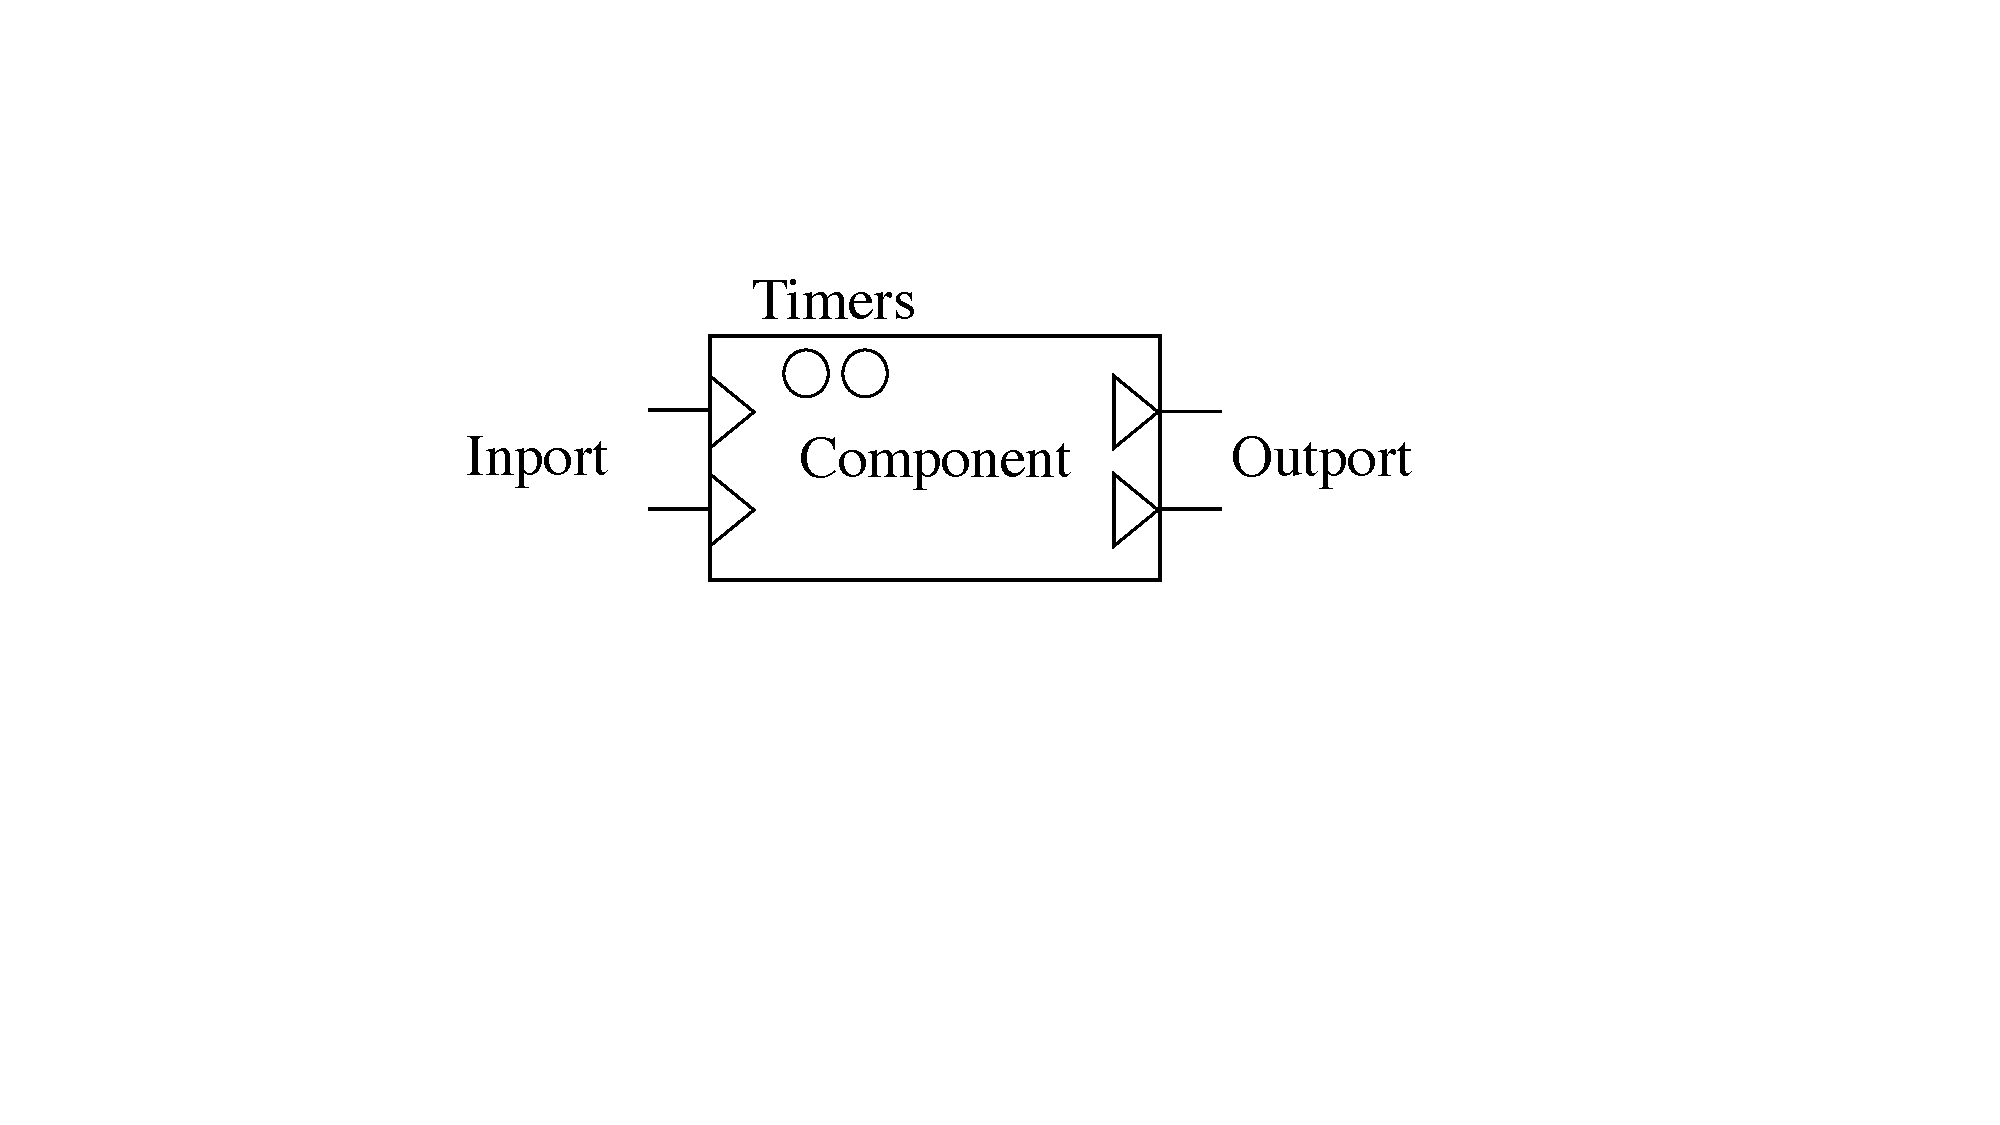
\epsfig{file=images/cost.pdf, width=7cm}
		\caption{COST component. While inports and outports allow to directly communicate with other components, timers trigger events specific to the component.}
		\label{fig:cost}
	\end{figure}	
	
	%%% Contributions
	\subsection{Contributions}
	In this document we describe the main features of the Komondor simulator and system model considerations, as well as some basic guidelines to run it. The main contributions done in this document are listed below:
	\begin{itemize}
%		\item \sergiost{We provide an} \sergio{O}verview of the first version of the Komondor simulator.
%		\item \sergiost{We describe} \sergio{Description of} the implementation done for each of the included functionalities, as well as the main considerations done.
%		\item \sergiost{We provide a} \sergio{S}et of validations that ensure the proper operation of the presented simulator.
%		\item \sergiost{We provide a} \sergio{T}utorial to allow an easy installation and execution of the simulator. Moreover, some implementation details are granted in case the reader is interested in extending the simulator.
		\item We provide an overview of the first version of the Komondor simulator.
		\item We describe the implementation done for each of the included functionalities, as well as the main considerations done.
		\item We provide a set of validations that ensure the proper operation of the presented simulator.
		\item We provide a tutorial to allow an easy installation and execution of the simulator. Moreover, some implementation details are granted in case the reader is interested in extending the simulator.
	\end{itemize}	
	
	Note, as well, that detailed technical information regarding code development is out of the scope of this document. Please, refer to the GitHub repository for more details on code implementation.
	
	%%%  Structure
	\subsection{Document Structure}
	\label{section:structure}
	This documents is structured as follows: Section \ref{section:system_model} describes the main design principles of Komondor. Then, Section \ref{section:mac_features} defines the implementation of IEEE 802.11 functionalities considered so far, which are validated in Section \ref{section:validations}. A tutorial and some development notes are provided in Section \ref{section:tutorial_and_development_notes}. Finally, some remarks are given in Section \ref{section:conclusions}.
	
%%%%%%%%%%%%%%%
% 2. SYSTEM MODEL
%%%%%%%%%%%%%%%
\section{Komondor Design Principles}
\label{section:system_model}
One of the main tasks regarding the implementation of Komondor relies on defining its design principles, which lay the foundations of the simulator. In this Section we describe the models defined for simulating the different communication aspects that a wireless device is intended to implement.
	
	%%% Channel Modeling
	\subsection{Channel Modeling}
	Channel modeling characterizes the signal propagation effects between the transmitter and the receiver. In order to be flexible and allowing to simulate different scenarios and casuistic, we define a set of path-loss and co-channel interference models, which are described next.
	
		% Path-loss
		\subsubsection{Path-loss Models}
		In order to provide the most representative wireless environments, we implemented the following set of path-loss models, which can be further extended by any developer:
		\begin{itemize}
			\item Free Space Path Loss (FSPL): a free-space model is considered, which captures direct line-of-sight and ignores shadowing effects. The experienced loss of power during a transmission that assumes this model is given by:
			\begin{equation}
				\text{FSPL} = 20 \log_{10}(d) + 20 \log_{10}(f) + 20 \log_{10}\Big(\frac{4\pi}{c}\Big) - G_t - G_r,
				\nonumber
			\end{equation}
			where $d$ is the distance between the transmitter and the receiver, $f$ is the frequency used in GHz, $c$ is the light speed in $m/s$, and $G_t$ and $G_r$ are the gains in dB at the transmitter and the receiver, respectively.
			\item Okumura-Hata model \cite{hata1980empirical}: this well-known model was conceived for predicting the path-loss of cellular transmissions in outside urban and rural environments. Since our main concern is related to dense urban areas, let the loss, $L_U$, be given by: 
			\begin{equation}
			\begin{aligned}
				L_U =  &69.55 + 22.16 \log_{10}(f) - 13.82 \log_{10} (h_B) + (44.9 - 6.55 \log_{10}(h_B)) \log_{10}(d) - \\ 
				& 3.2 \log_{10}(11.7554 h_M)^2 - 4.97,
			\end{aligned}
			\nonumber
			\end{equation}
			where $f$ is the center frequency in MHz, $h_B$ is the height of the transmitter antenna, $d$ is the distance between the transmitter and the receiver in meters, and $h_M$ is the height of the receiver's antenna.
			\item Indoor model: this model represents a simple indoor scenario, which is useful to simulate typical scenarios such as flats, schools or restaurants. According to this model, the loss, $L_{indoor}$, experienced during a transmission is:		
			\begin{equation}
				L_{indoor} = \text{PL}_f + 10 \alpha \log_{10}(d) + h_s + \Big(\frac{d}{f_w}\Big) h_o,
				\nonumber
			\end{equation}
			where $\text{PL}_f$ is the path-loss factor, $\alpha$ is a constant that depends on the propagation model, $d$ is the distance in meters between the transmitter and the receiver, $h_s$ is the shadowing factor, $f_w$ is the frequency of walls, and $h_o$ is the obstacles factor.
			
			Furthermore, a variation of this path-loss model is provided, in order to introduce random variables that determine the shadowing and obstacles effects in the power losses.
			\item Residential path-loss model IEEE 802.11ax: such model is included in the 11ax amendment, and captures the path-loss effects of a typical apartments building. The loss, $L_{indoor-ax}$, experienced during a transmission is given by:
			\begin{equation}
				\begin{aligned}
				L_{indoor-ax} = &40.05 + 20 \log_{10}\Big(\frac{f_c}{2.4}\Big) + 20 \log_{10}(\min(d,5)) + (d>5)  35 \log_{10}\Big(\frac{d}{5}\Big) + \\
				&18.3 F^{\frac{F+2}{F+1}-0.46} + 5 W,
				\end{aligned}
				\nonumber
			\end{equation}

			where $f_c$ is the frequency in GHz, $d$ is the distance between the transmitter and the receiver, $F$ is the number of floors traversed, and $W$ is number of walls traversed in the x-direction plus the number of walls traversed in the y-direction
		\end{itemize}	
	
		% Co-channel interference
		\subsubsection{Adjacent Channel Interference Models}
		In addition to the introduced path-loss types, it is important to take into account the Adjacent Channel Interference (ACI), which conditions the interaction between devices. The fact of using non-overlapping channels entails more aggressive interactions given that devices in other channels also contribute to the sensed interference in a given receiver. An example of channels overlapping is shown in Figure \ref{fig:cochannel_interference}.
		\begin{figure}[h!]
			\centering
			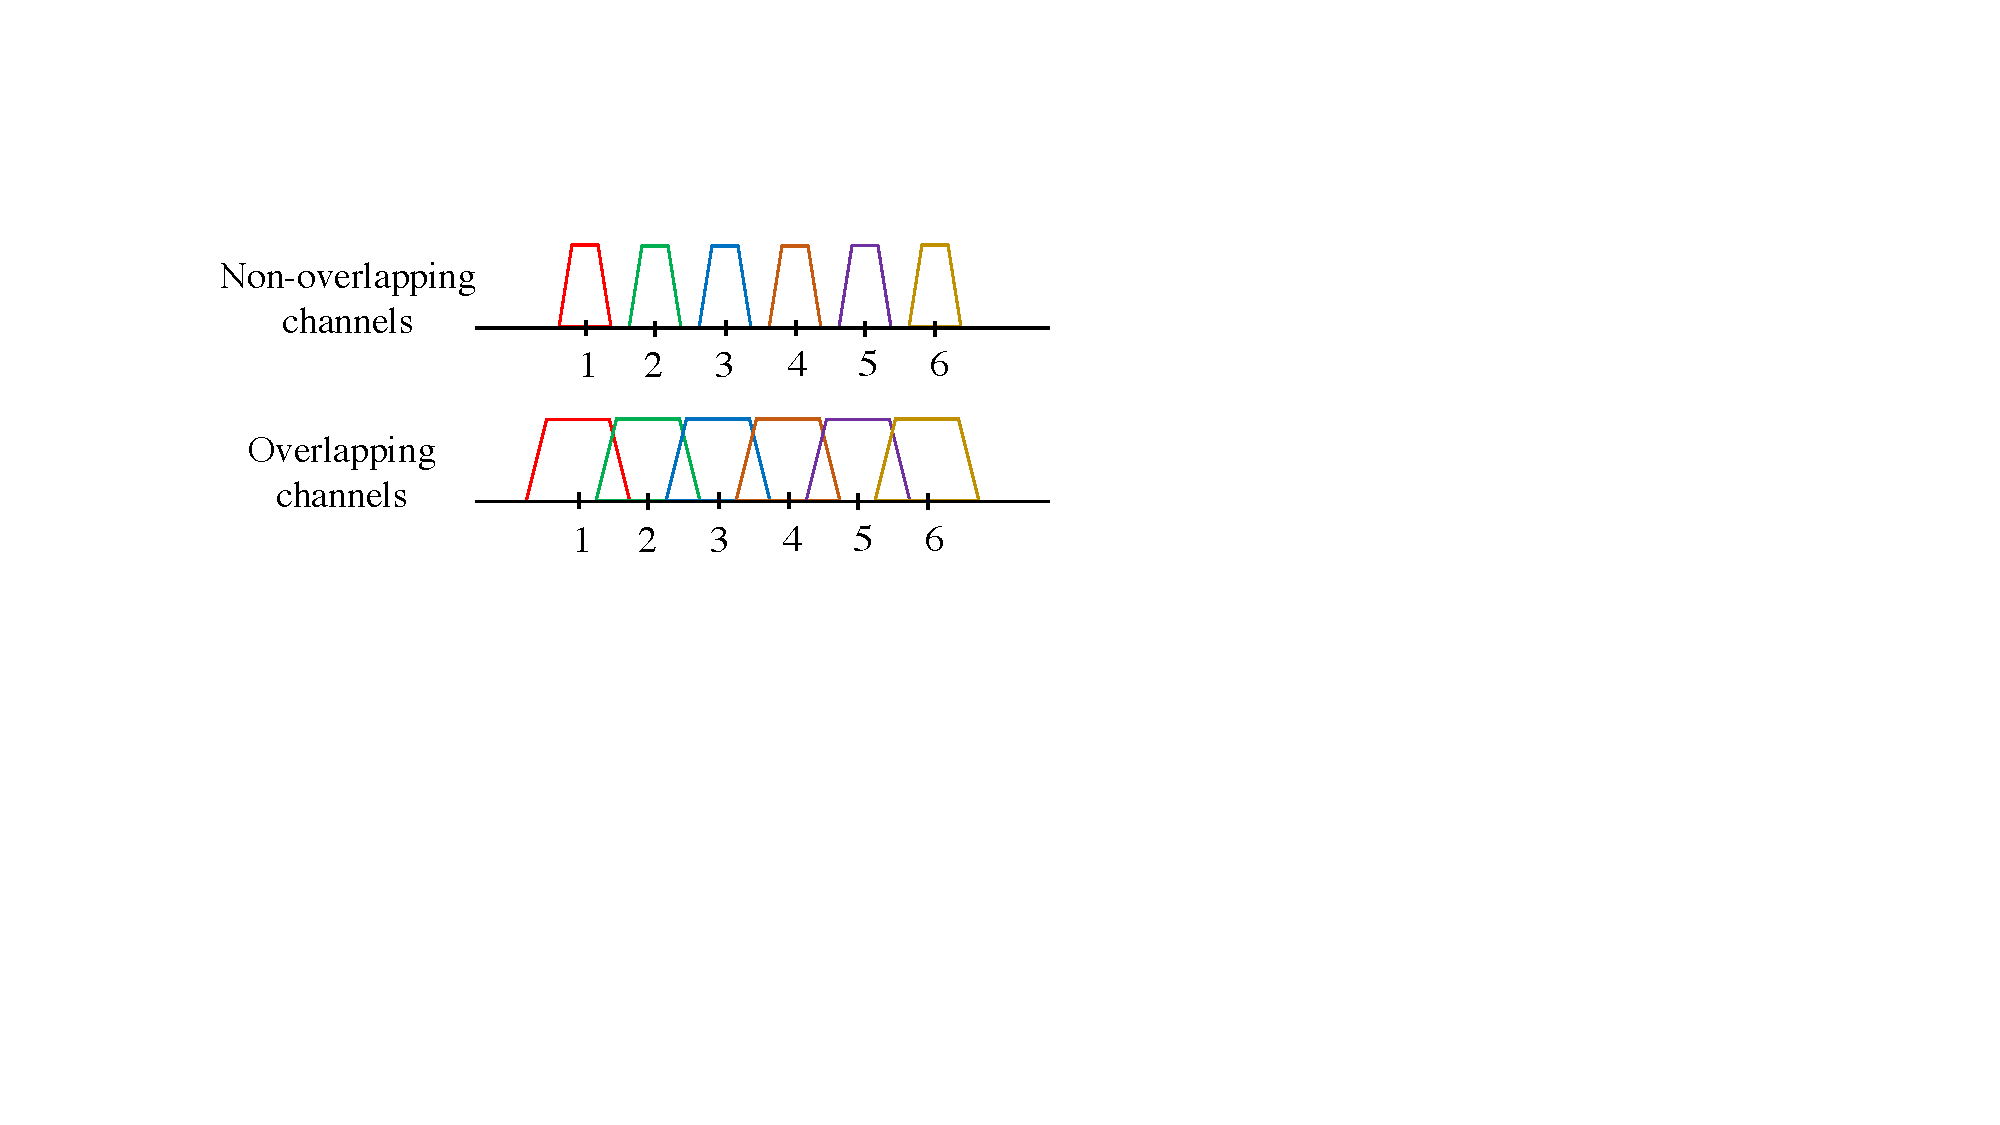
\epsfig{file=images/cochannel_interference.pdf, width=9cm}
			\caption{Channel models with and without ACI}
			\label{fig:cochannel_interference}
		\end{figure}	
		
		In particular, Komondor includes the following ACI models:		
		\begin{itemize}
			\item \textbf{No interference}: no power is leaked to adjacent channels.
			\item \textbf{Total interference}: power from other channels is leaked, so that a 20 dB decrease is noticed for each channel distance. For instance, the power that channel 1 leaks into channel 3 is the actual power in channel 1 minus 40 dBr. 
			\item \textbf{Limited interference}: in this case, only immediate adjacent channels leak power to the target one, so that a 20 dB decrease is noticed from consecutive channels.
		\end{itemize}
				
		A critical assumption done in Komondor is that the incoming power in a given receiver is assumed to be the same during the entire transmission. This relaxation allows us to easily determine whenever the channel of interest is busy or not. A direct implication of it affects to path-loss models used, as well as some of them assume random variations of the medium, preventing to obtain the same result with different power received calculations (so far, power received is added and subtracted when the node accesses and leaves the channel, respectively). Thus, for each node, Komondor stores the incoming power of a given transmission when it begins and subtracts the power when it is over. 
	
	%%% Traffic modeling
	\subsection{Traffic Modeling}
	\label{section:traffic_modelling}
	Traffic modeling refers to the capacity of generating data in higher transmission layers. So far, Komondor only considers downlink traffic, so that data transmissions are initiated by APs. Regarding traffic generation, we have considered three different models:
	\begin{itemize}
		\item \textbf{Full buffer}: transmitters are in a permanent saturation regime, so that they always have packets to be sent.
		\item \textbf{Poisson}: packets are generated according to a Poisson distribution process, so that the average time between packets is determined by the packet generation rate $\lambda$, and which is given by $\Delta_{\rm p} = \frac{1}{\lambda}$.
		\item \textbf{Deterministic}: packets are generated at fixed time intervals given by the packet generation rate, $\Delta_{\rm d} = 1/\lambda$.
	\end{itemize}

	Figure \ref{fig:traffic_models} illustrates the aforementioned traffic models. 
	\begin{figure}[h!]
		\centering
		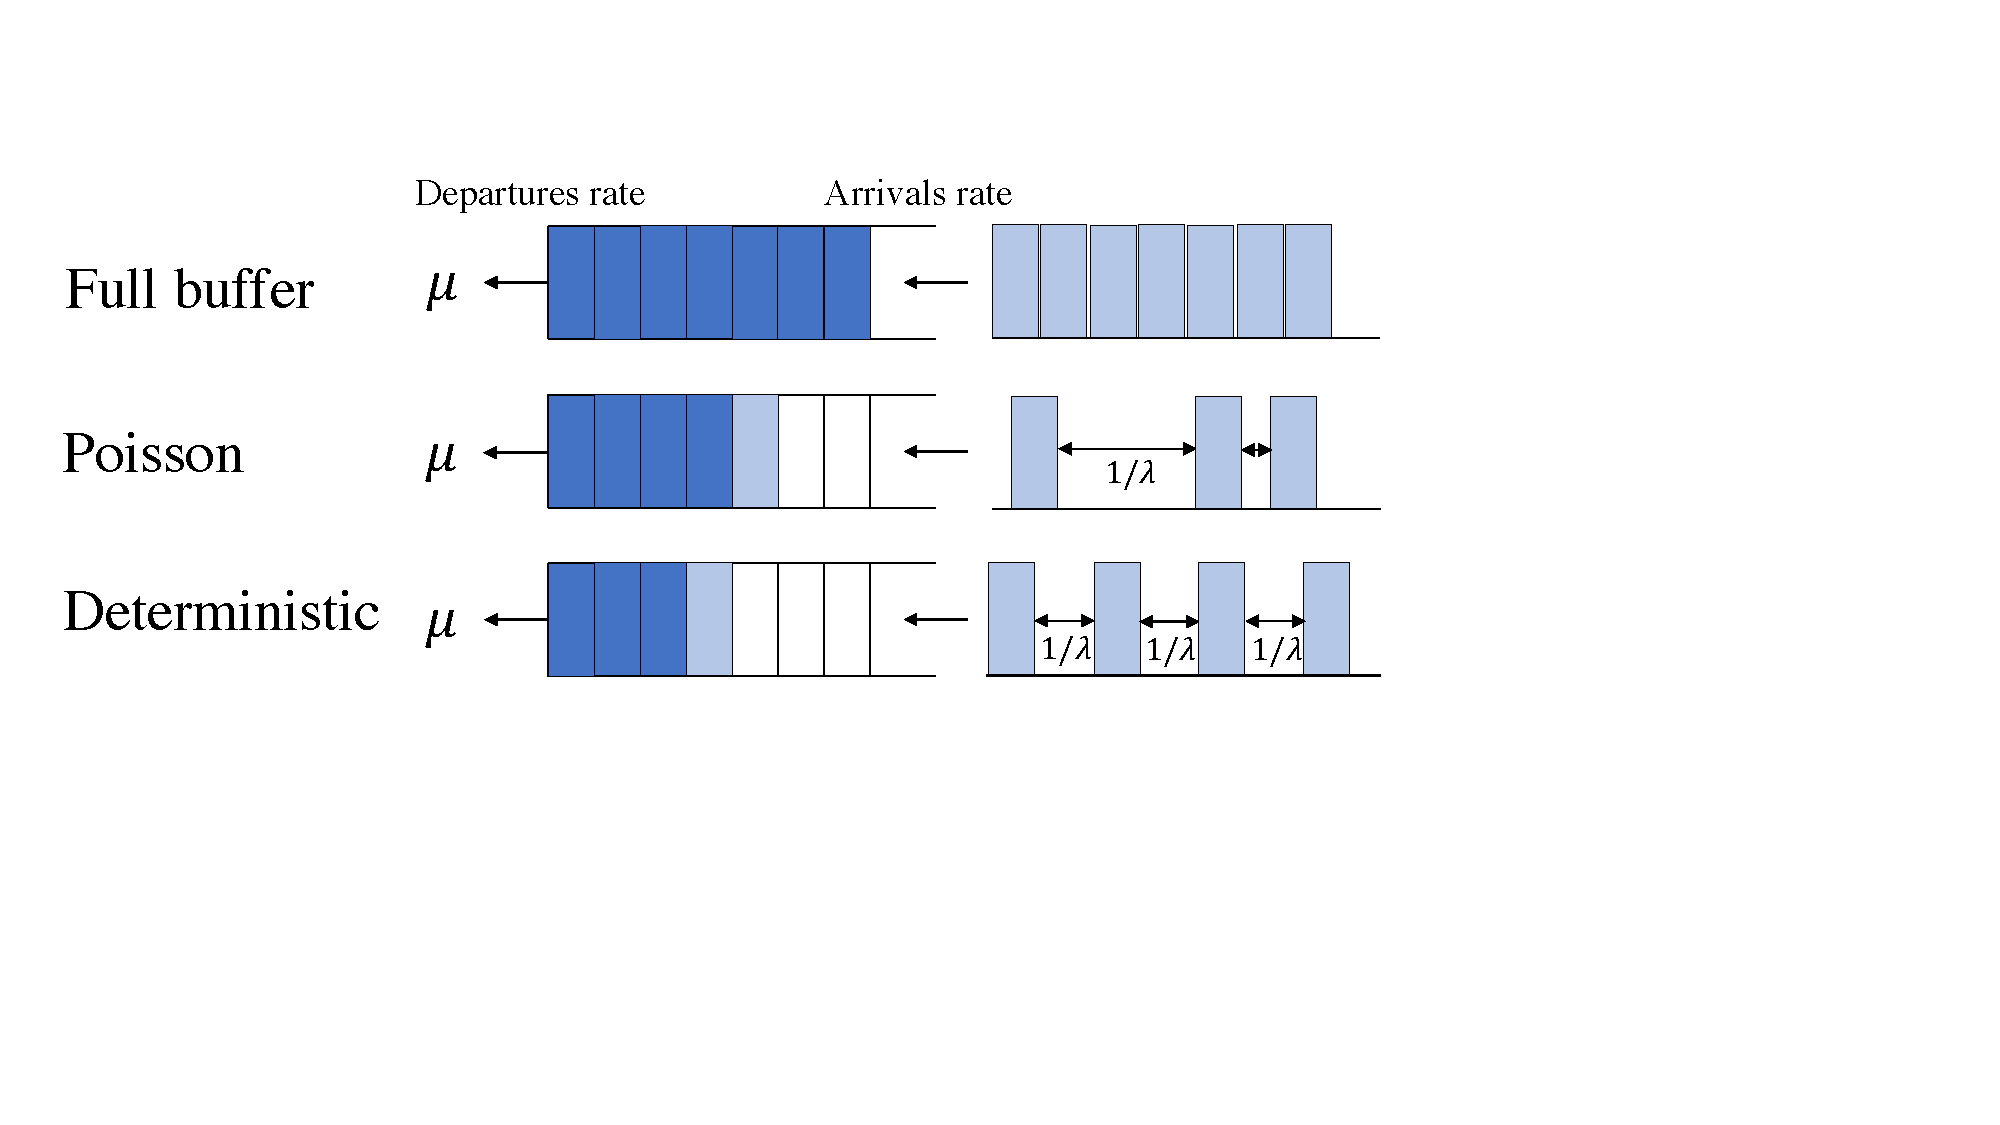
\epsfig{file=images/traffic_models.pdf, width=9cm}
		\caption{Traffic models used in Komondor}
		\label{fig:traffic_models}
	\end{figure}	
	
	%%% Data rate modeling
	\subsection{Link Modeling}
	In order to determine the data rate to be used during a given transmission, the MCS table defined in the IEEE 802.11ax is considered. Komondor assumes that the MCS used between a pair of devices is determined by the SINR at the receiver, so that the maximum allowable MCS is used. The required SINR that corresponds to each MCS is defined in Table \ref{table:sinr_thresholds_mcs}, as well as the granted data rate for each channel width.
	% MCS IEEE 802.11ax
	\begin{table}[]
		\centering
		\resizebox{\textwidth}{!}{\begin{tabular}{|c|c|c|c|c|c|c|c|}
			\hline
			\multirow{2}{*}{\textbf{\begin{tabular}[c]{@{}c@{}}MCS \\ index\end{tabular}}} &
			\multirow{2}{*}{\textbf{\begin{tabular}[c]{@{}c@{}}SINR \\ interval (dBm)\end{tabular}}} &
			\multirow{2}{*}{\textbf{\begin{tabular}[c]{@{}c@{}}Modulation\\ type\end{tabular}}} & \multirow{2}{*}{\textbf{\begin{tabular}[c]{@{}c@{}}Coding\\ rate\end{tabular}}} & \multicolumn{4}{c|}{\textbf{Data rate (Mbps)}} \\ \cline{5-8} 
			& &  &  & \textbf{20 MHz} & \textbf{40 MHz} & \textbf{80 MHz} & \textbf{160 MHz} \\ \hline
			0 & {[}-82, -79) & BPSK & 1/2 & 4 & 8 & 17 & 34 \\ \hline
			1 & {[}-79, -77) & QPSK & 1/2 & 16 & 33 & 68 & 136 \\ \hline
			2 & {[}-77, -74) & QPSK & 3/4 & 24 & 49 & 102 & 204 \\ \hline
			3 & {[}-74, -70) & 16-QAM & 1/2 & 33 & 65 & 136 & 272 \\ \hline
			4 & {[}-70, -66) & 16-QAM & 3/4 & 49 & 98 & 204 & 408 \\ \hline
			5 & {[}-66, -65) & 64-QAM & 2/3 & 65 & 130 & 272 & 544 \\ \hline
			6 & {[}-65, -64) & 64-QAM & 3/4 & 73 & 146 & 306 & 613 \\ \hline
			7 & {[}-64, -59) & 64-QAM & 5/6 & 81 & 163 & 340 & 681 \\ \hline
			8 & {[}-59, -57) & 256-QAM & 3/4 & 98 & 195 & 408 & 817 \\ \hline
			9 & {[}-57, -54) & 256-QAM & 5/6 & 108 & 217 & 453 & 907 \\ \hline
			10 & {[}-54, -52) & 1024-QAM & 3/4 & 122 & 244 & 510 & 1021 \\ \hline
			11 & $\geq$ 52 & 1024-QAM & 5/6 & 135 & 271 & 567 & 1143 \\ \hline
		\end{tabular}}
		\caption{Data rates granted per MCS in IEEE 802.11ax. Guard Intervals (GI) of 1600 ns are only considered.}
		\label{table:sinr_thresholds_mcs}	
	\end{table}
	
	So far, link adaptation is not considered\footnote{Future work contemplates the inclusion of Minstrel as a rate adaptation scheme.}. Instead, the MCS to be used between each transmitter-receiver pair is negotiated at the beginning of the first transmission, which remains static throughout all the simulation. In practice, the highest possible modulation is computed between each transmitter-receiver pair according to the SINR at the receiver.
		
	Finally, regarding the transmission time for sending a packet, it is computed as a function of the data rate and the size of the packet to be transmitted. Packet lengths are defined according to the IEEE 802.11ax specification, which is further described in Section \ref{section:parameters}.

	%%% Collisions model
	\subsection{Collisions Modeling}
	Collisions are critical to be implemented because they determine the actual performance in a given network, thus allowing to capture situations that may occur in real environments. In particular, packet losses mostly occur because two nodes transmit at the same time (their backoff reaches 0 simultaneously) hidden-node effects or link asymmetries. An example of a hidden-node collision is shown in Figure \ref{fig:collisions_hidden_node}, in which nodes A and C transmit simultaneously to B because they do not sense the other's transmission.	The resulting interference may lead into a collision and provoke that none of the packets can be properly decoded.
	\begin{figure}
		\centering
		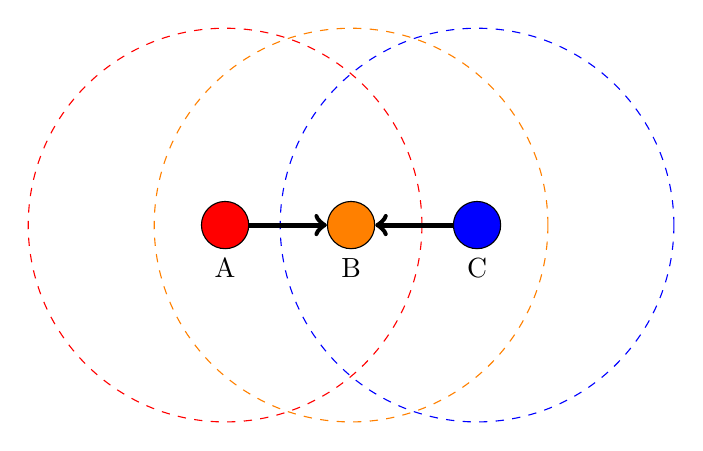
\begin{tikzpicture}
		\node at (0,0) [circle, fill=red, draw, minimum width=0.6cm,minimum height=0.6cm, label=below:$\text{A}$] (A) {};
		\node at (A) [circle,draw=red, minimum size=5cm, dashed] (Ac) {};
		\node[circle, fill=orange, draw, minimum width=0.6cm,minimum height=0.6cm, label=below:$\text{B}$] (B) [right of=A, xshift=0.6cm] {};
		\node at (B) [circle,draw=orange, minimum size=5cm, dashed] (Bc) {};
		\node[circle,draw, fill=blue, minimum width=0.6cm,minimum height=0.6cm, label=below:$\text{C}$] (C) [right of=B, xshift=0.6cm] {};
		\node at (C) [circle,draw=blue, minimum size=5cm, dashed] (Cc) {};      
		\draw [->,line width=1.8pt] (A) edge (B) (C) edge (B);
		\end{tikzpicture}
		\caption{Hidden-node cause of collision} \label{fig:collisions_hidden_node}
	\end{figure}

	In Komondor, a packet loss is considered when the ACK timeout expires at a given transmitter. However, it is critical to identify what caused such loss, which may allow to further analyze the issue. In particular, Komondor is able to categorize packet losses as follows:
	\begin{itemize}
		\item \textbf{PACKET\_LOST\_DESTINATION\_TX}: packet is discarded because the destination was already transmitting when the packet transmission was attempted. In this case we know that the transmitter could not listen to the receiver at the moment of starting a transmission.
		\item \textbf{PACKET\_LOST\_LOW\_SIGNAL}: the packet cannot be decoded because the signal strength is not enough (i.e., it is less than the CCA).
		\item \textbf{PACKET\_LOST\_INTERFERENCE}: packet is lost due to interference sensed at the receiver, which does not accomplish the capture effect condition.	
		\item \textbf{PACKET\_LOST\_PURE\_COLLISION}: packet is lost because two nodes transmit to the same destination, so that both signal strengths are high enough to be decoded  at the receiver (the situation shown in Figure \ref{fig:collisions_hidden_node}).
		\item \textbf{PACKET\_LOST\_LOW\_SIGNAL\_AND\_RX}: the destination is already receiving data when a new data transmission starts. However, the newest signal strength is not high enough to be decoded in normal conditions. This event comprises the abovementioned PACKET\_LOST\_DESTINATION\_TX and PACKET\_LOST\_LOW\_SIGNAL causes.
		\item \textbf{PACKET\_LOST\_RX\_IN\_NAV}: packet is lost because the target node is in a NAV period (it previously decoded an RTS/CTS sequence).		
		\item \textbf{PACKET\_LOST\_BO\_COLLISION}: the packet is lost because a backoff collision occurred (i.e., two or more interfering devices ended their backoff simultaneously), provided that the interfering signal is strong enough to cause a collision.
	\end{itemize}	
	
%	Furthermore, other types of collisions that are uncontrolled may occur. For instance, when applying Channel Bonding, the situation depicted in Figure \ref{fig:boat1} may occur.
%	\begin{figure}[h!]
%		\centering
%		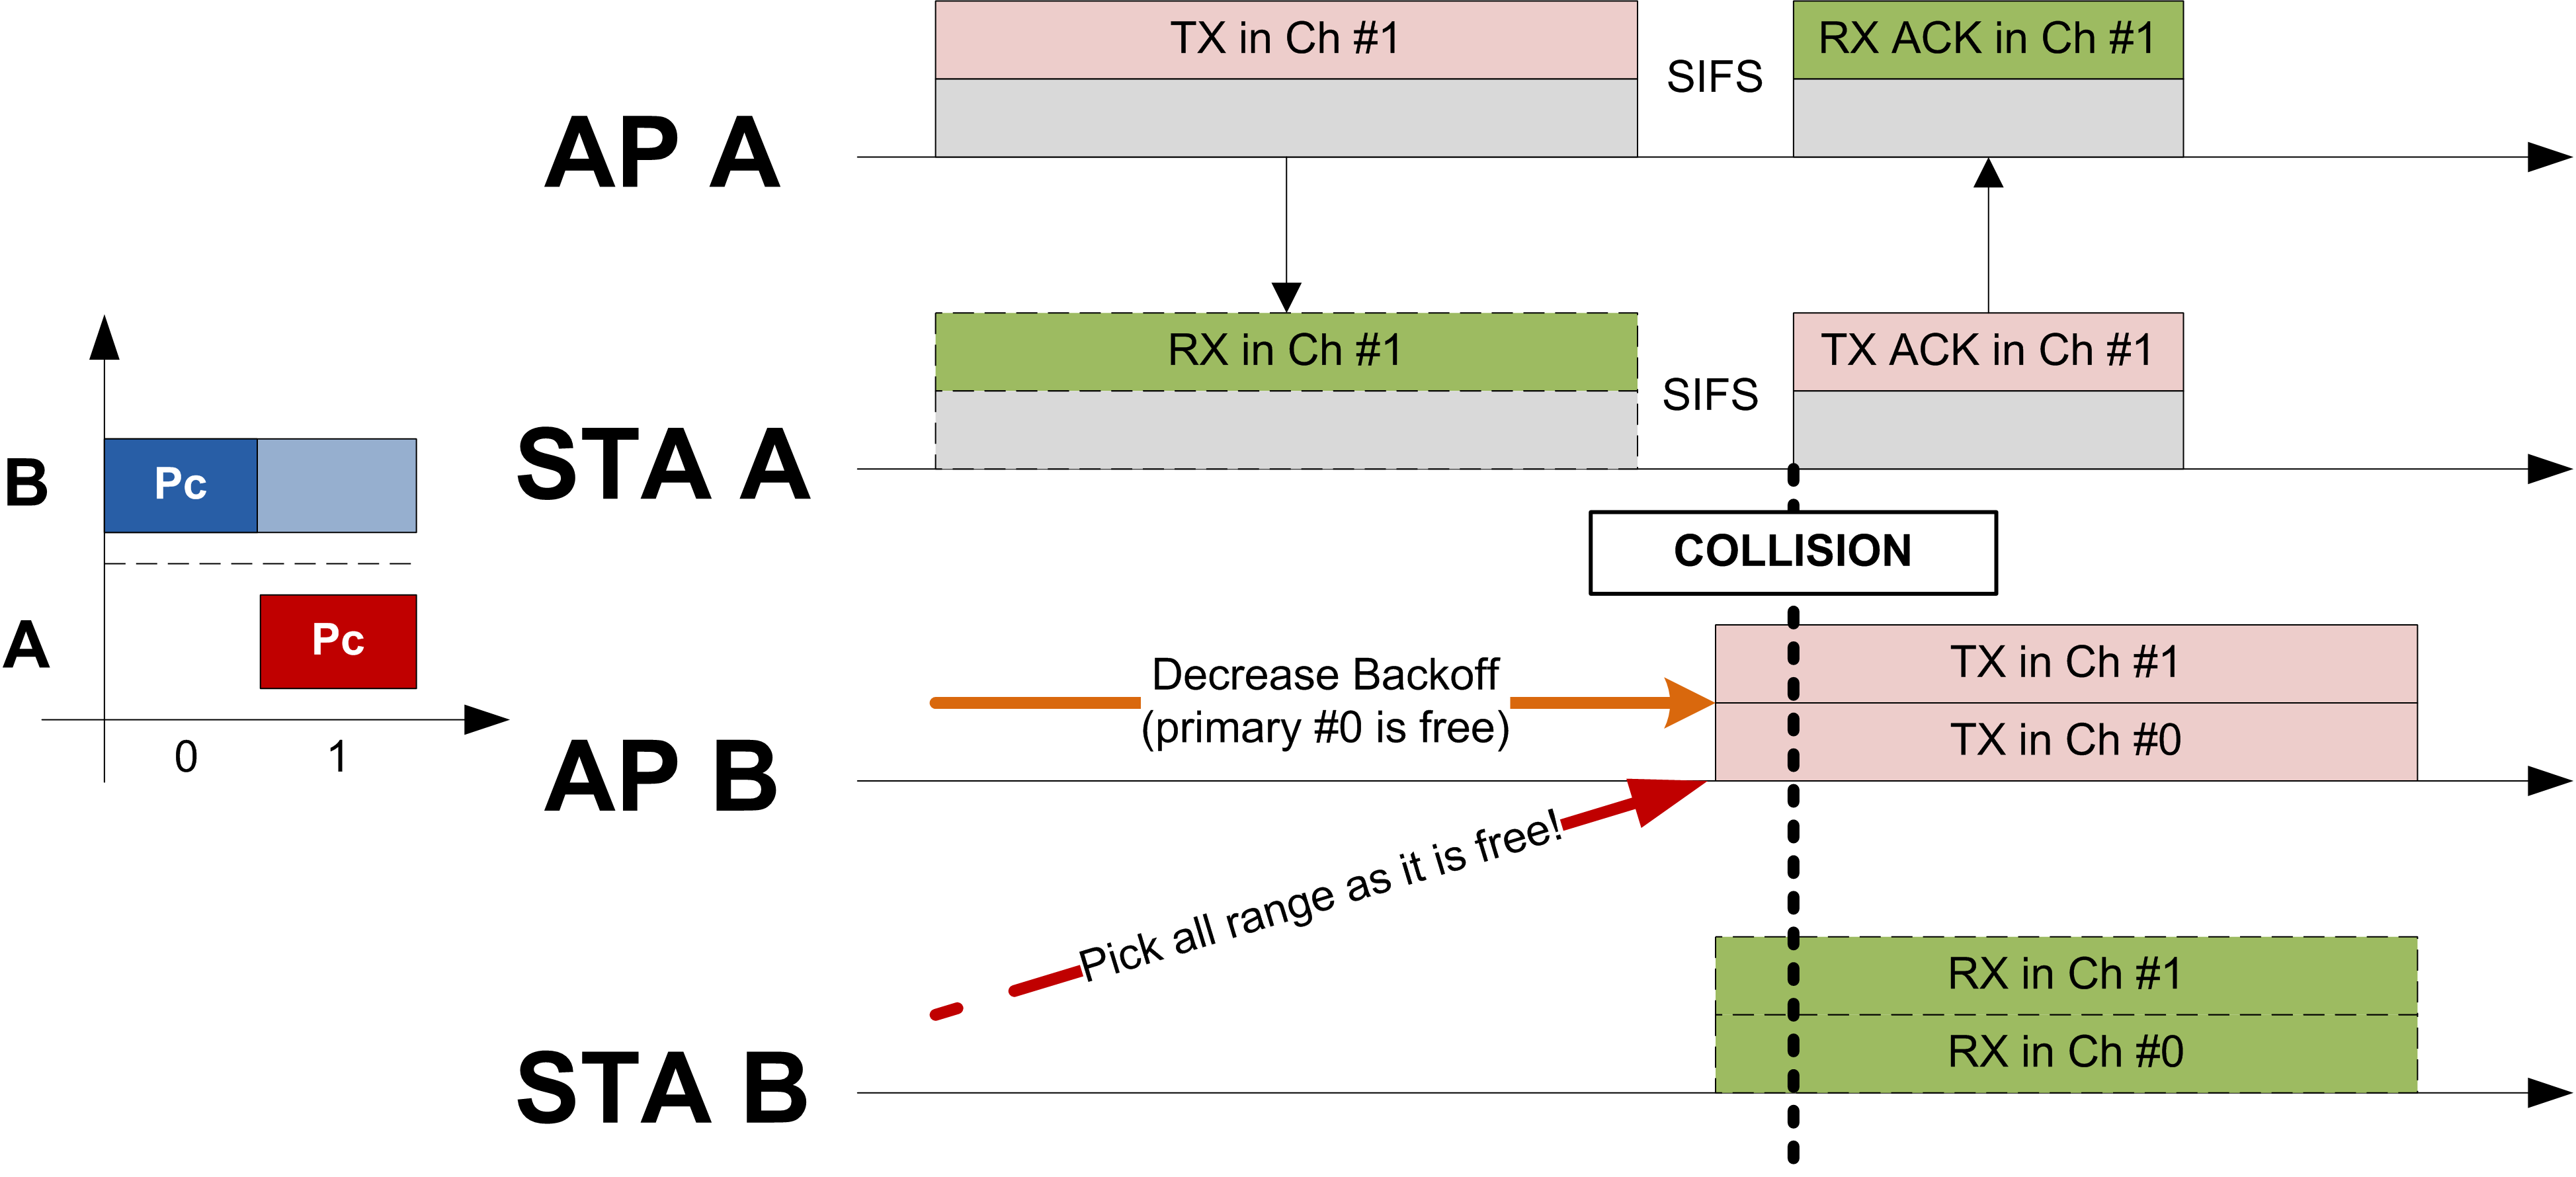
\includegraphics[scale=0.7]{images/ACK_issue.png}
%		\caption{Weird case when collisions occur due to last transmitting AP checks the channel right in the SIFS period of other WLAN and picks a range affecting the previous transmission.}
%		\label{fig:boat1}
%	\end{figure}

%%%%%%%%%%%%%%%
% MAC FEATURES
%%%%%%%%%%%%%%%
\section{IEEE 802.11 Features}
\label{section:mac_features}
In this Section we provide an overview of the main MAC layer features included in Komondor, so that their practical implementation can be further understood.
	
	%%% Channel Access
	\subsection{Channel Access}
	\label{section:channel_access}
	When a wireless device has a packet to be sent, it employs DCF to access the medium, which makes use of CSMA/CA and BEB. With that, transmissions are carried out if the target channel has been empty for a given Backoff (BO) time, which is computed according to a dynamic CW. A channel is considered to be empty if the interference in it is lower than a Clear Channel Assessment (CCA) threshold. Furthermore, a packet transmission is successful whenever the receiver SINR is equal or higher than the Capture Effect (CE) threshold, which allows defining the rate at which packet losses occur, regardless on the Modulation Coding Scheme used.
		
		% DCF
		\subsubsection{Distributed Coordination Function}
		\label{section:dcf}		
		As previously mentioned, the CSMA/CA operation is based on the DCF, which orchestrates channel access in a distributed manner. Roughly, transmitters (e.g., devices that have data to be transmitted) choose a random BO value, which is decremented only if the channel is sensed as idle due to the CCA condition. Otherwise, the BO is paused and the transmission is delayed. Figure \ref{fig:dcf_operation} shows an example of the DCF operation in which three nodes listen to each other in the same wireless scenario. As it is shown, STA2 wins the channel access because its initial BO timer is the lowest one. During the packet transmission, STA1 listens the channel busy and stops its BO operation. Once data transmission is finished and the channel has been idle for a DIFS interval, the BO procedure is activated in all the devices that have a packet to be transmitted and sense the channel idle.
		\begin{figure}[h!]
			\centering
			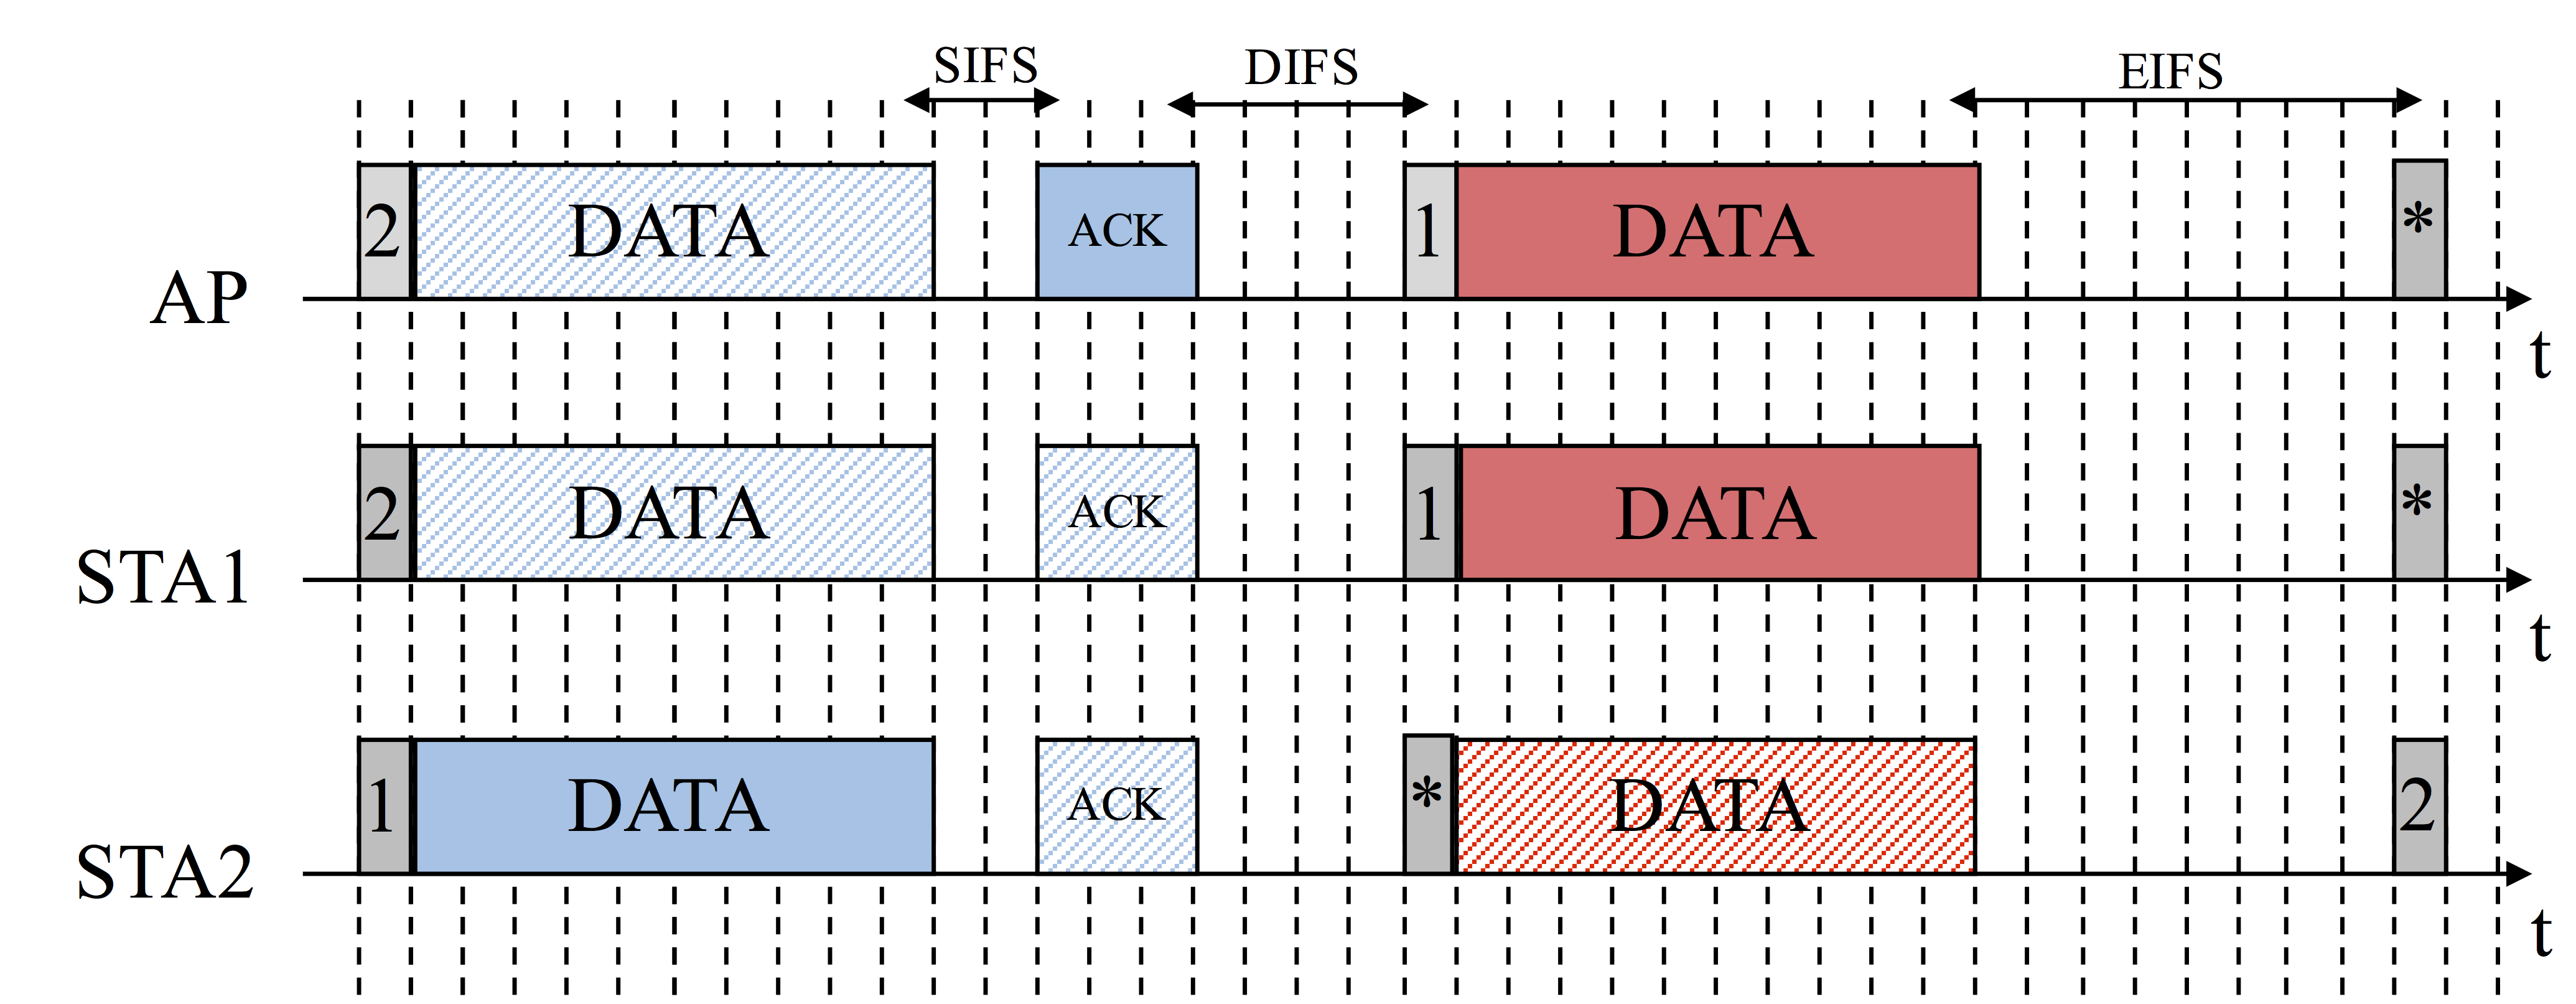
\epsfig{file=images/dcf_operation, width=12cm}
			\caption{Example of the DCF procedure}
			\label{fig:dcf_operation}
		\end{figure}
		
		Regarding BEB, it determines the process of generating the BO, which depends on the Contention Window (CW). The CW is dynamically adapted on a per-packet basis, so that the CW increases or decreases according to successful/failed transmissions. Given a minimum and a maximum boundaries for CW ($\rm CW_{\rm min}$ and $\rm CW_{\rm max}$, respectively), the reset operation is performed when a successful transmission is carried out. In such situation, the CW is set to $\rm CW_{\rm min}$. Otherwise, when packet losses occur, the CW is increased without exceeding $\rm CW_{\rm max}$. To do so, a counter (namely $\rm CW_{\rm count}$) is maintained and increased one unit each time a packet loss occurs. Then, the CW is computed as $\rm CW = \rm CW_{\rm min} \times 2^{\rm CW_{\rm count}}$.
		
		Furthermore, Komondor provides two different ways of computing the BO value as a function of the CW:
		\begin{itemize}
			\item \textbf{Uniform}: the generated BO is a number between 0 and $\text{CW}-1$, and all the values have the same probability.
			\item \textbf{Exponential}: instead of using an uniform distribution, we use an exponential one, so that the generated BO is given by the mean CW value ($\frac{\text{CW}-1}{2}$).
		\end{itemize}
				
		An important consideration with respect to the discrete BO implementation considered in Komondor, is that devices are synchronized, which allows reproducing collisions by BO that depend on the congestion window and the number of coexisting nodes.
		
%		% CW Adaptation	
%		\subsubsection{Contention Window Adaptation}
%		\label{section:cw_adaptation} 
		
		% CE
		\subsubsection{Capture Effect}
		\label{section:capture_effect}
		In order to successfully decode the signal received, a receiver must perceive that the desired signal strength is bigger than a CE threshold, so that the received data can be distinguished among noise and interference present in the channel. Komondor considers an \emph{stronger-first} interference pattern for the data exchange process. Henceforth, a data packet is properly decoded only if posterior transmissions do not generate high enough interference to discard it. Note that a dominant data transmission is not going be considered at a given receiver that is already receiving any type of data from another node. In such case, both transmissions are considered to be lost. The stronger-first CE principle is shown in Figure \ref{fig:capture_effect}. 
		\begin{figure}[h!]
			\centering
			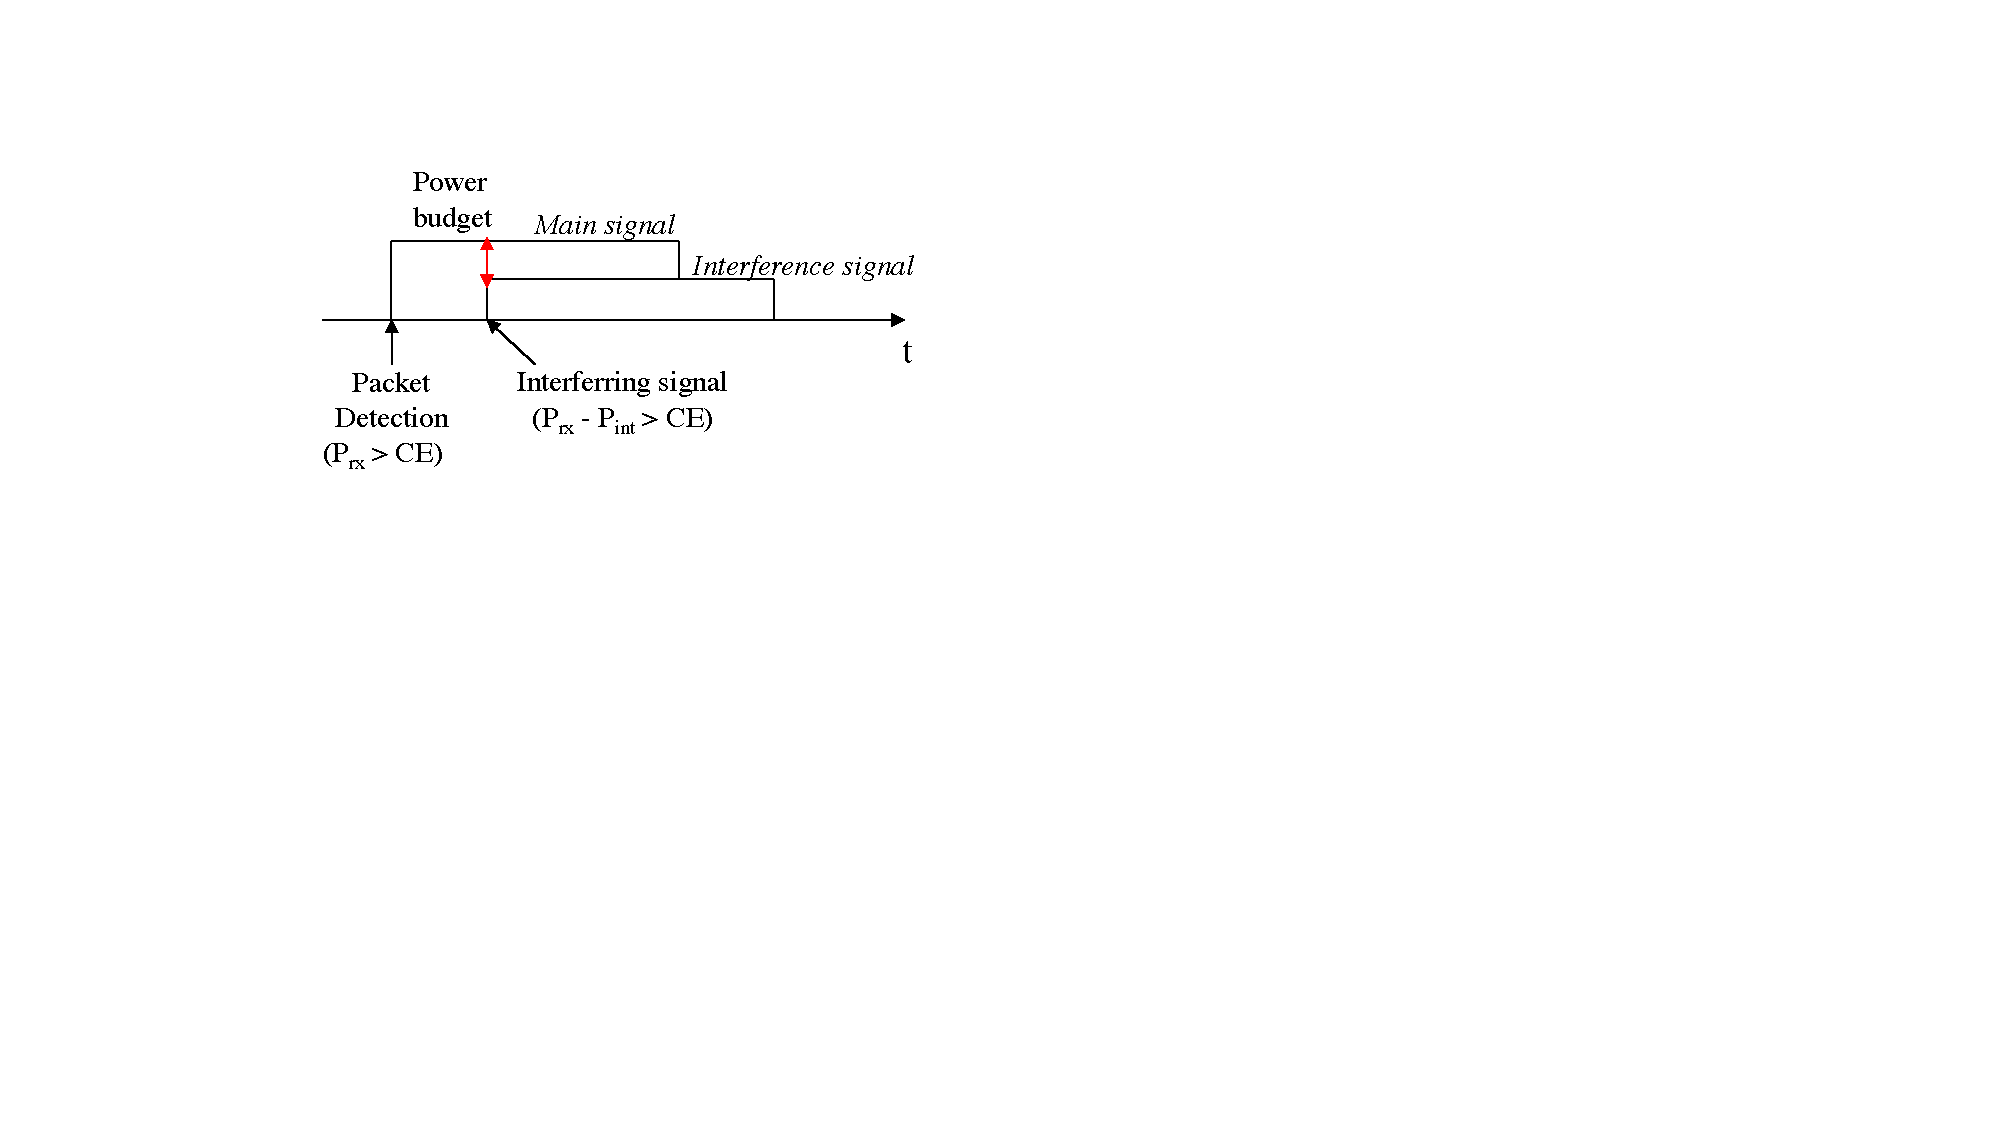
\epsfig{file=images/capture_effect, width=9cm}
			\caption{Stronger-First Capture Effect example}
			\label{fig:capture_effect}
		\end{figure}
	
	%%% RTS/CTS
	\subsection{RTS/CTS and NAV Allocation}
	The RTS/CTS mechanism is implemented in order to minimize the collisions by hidden node. Through RTS/CTS, transmitting nodes attempt to block the channel for the duration of their transmissions. For that, they send RTS packets and wait for confirmation about the clearness of the channel from the receivers' point of view. Through such packet exchange, overlapping nodes must set a virtual carrier sensing during the transmission duration, which allows reducing the collisions by hidden node. The RTS/CTS operation is exemplified in Figure \ref{fig:rts_cts_mechanism}. The scenario shown in Figure \ref{fig:collisions_hidden_node} is considered, so that the AP is the middle and both STAs do not sense each other.
	\begin{figure}[h!]
		\centering
		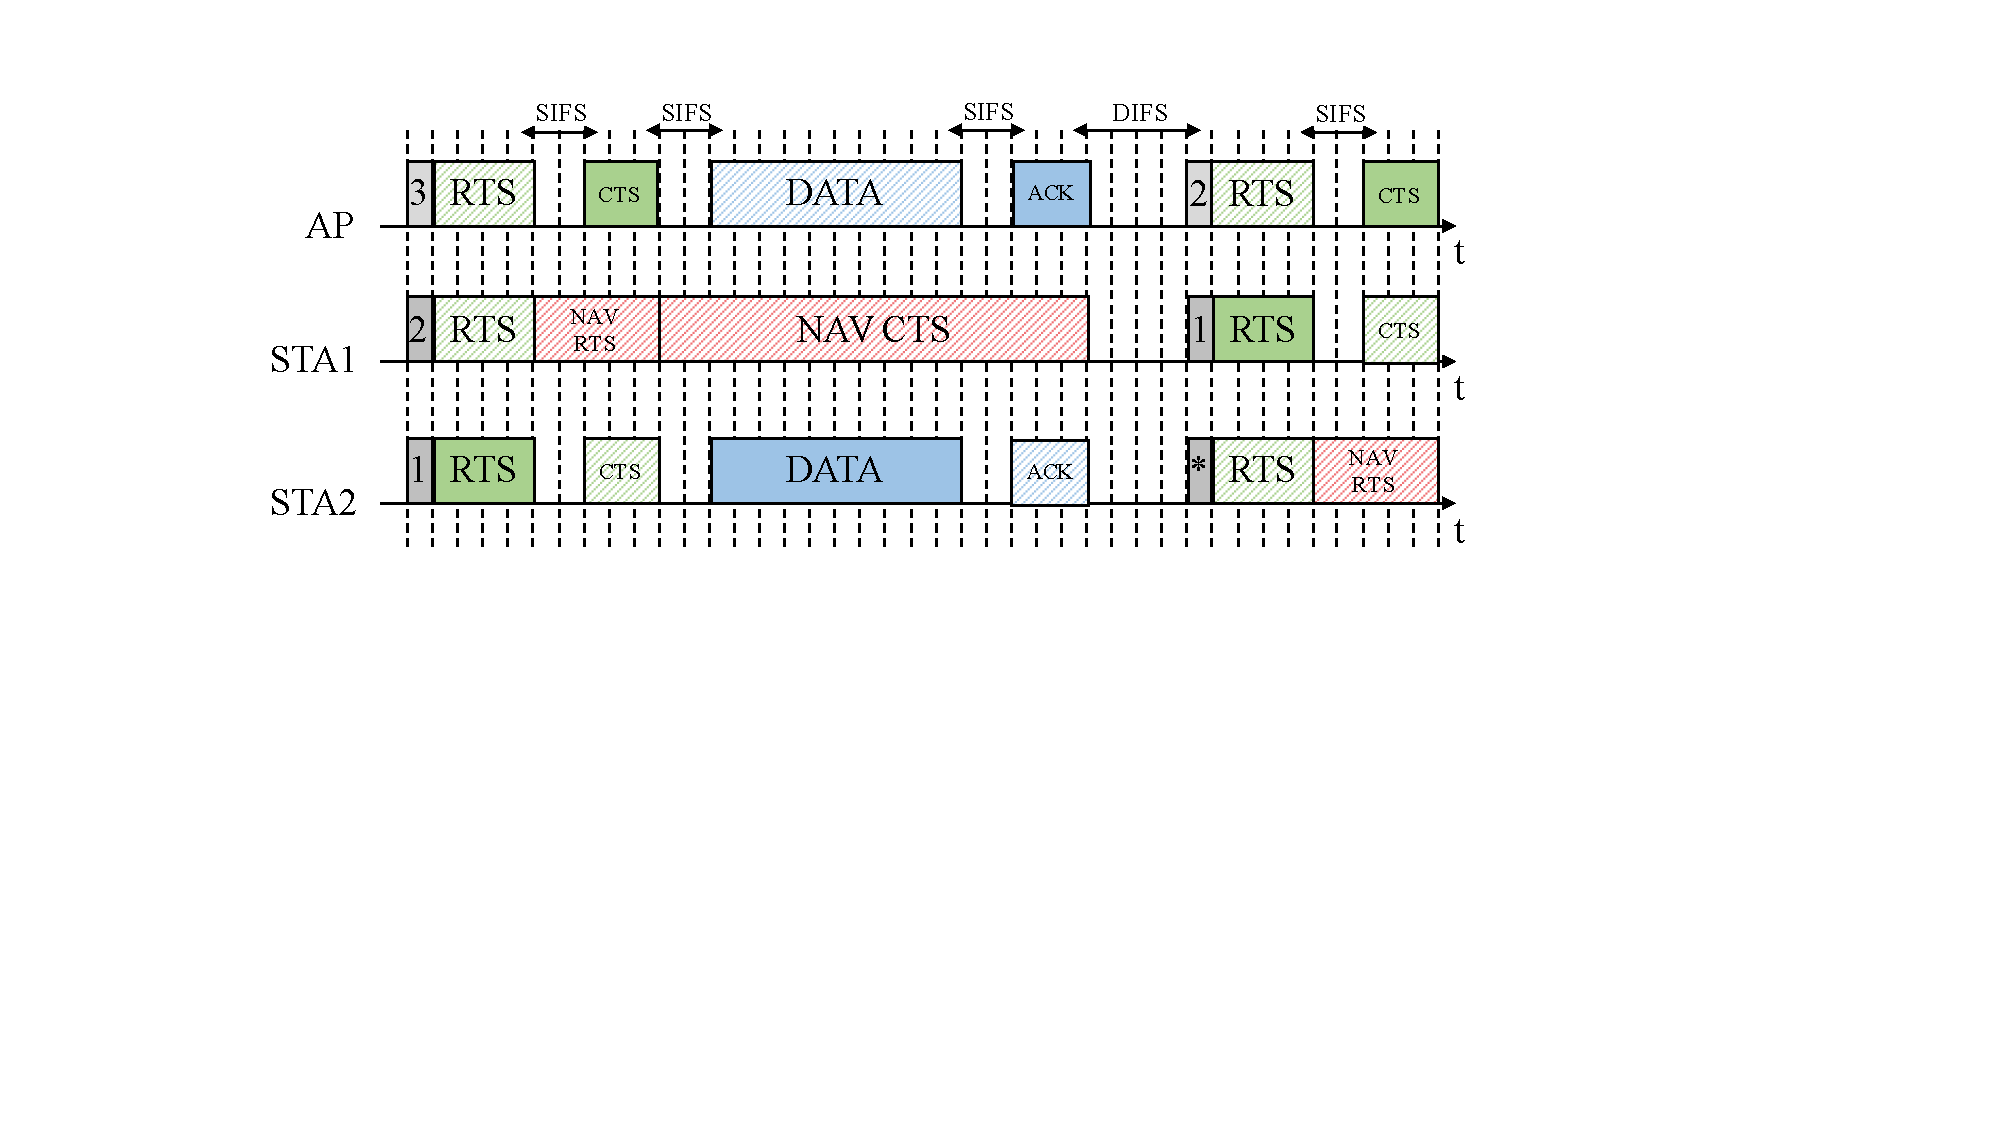
\epsfig{file=images/rts_cts_mechanism.pdf, width=12cm}
		\caption{Example of RTS/CTS implementation. The transmitter (STA2) sends an RTS packet before starting a transmission. The receiver (AP) answers with a CTS as it senses the channel free. The other coexisting devices (STA1) that listen either the RTS and/or the CTS, set their NAV accordingly.}
		\label{fig:rts_cts_mechanism}
	\end{figure}	
		
	%%% Channel Bonding
	\subsection{Channel Bonding}
	\label{section:channel_bonding}

	Dynamic channel bonding (DCB) is one of the most promising techniques to enhance spectral efficiency in IEEE 802.11ax WLANs, since it aims to make the most of the medium by transmitting data over several contiguous basic channels. For that, different DCB policies are implemented in Komondor, which can be interchangeably applied by the simulated WLANs. To perform DCB, one may explicitly define the available range of basic channels for each WLAN. Then, the following policies can be applied:
	\begin{itemize}
		\item \textbf{Only Primary (OP)}: the legacy operation is performed, so that only the primary channel is attempted to be accessed. This policy is also known as single-channel.
		\item \textbf{Static Channel Bonding (SCB)}: carrier sensing is performed at the primary channel. However, when attempting to transmit, all the channels within the CB range must be clear. Otherwise, a new backoff is computed.
		\item \textbf{Always-max (AM)}:\footnote{Some papers in the literature use the terms DCB and AM indistinctly. In this document we notate AM as an special case of DCB.} picks the widest possible channel found free for transmitting. Note that, in order to include secondary basic channels for transmitting, a WLAN must listen them free during at least a PIFS period before the backoff counter terminates as shown in Figure \ref{fig:dcb_dcf}.
		\begin{figure}
			\centering
			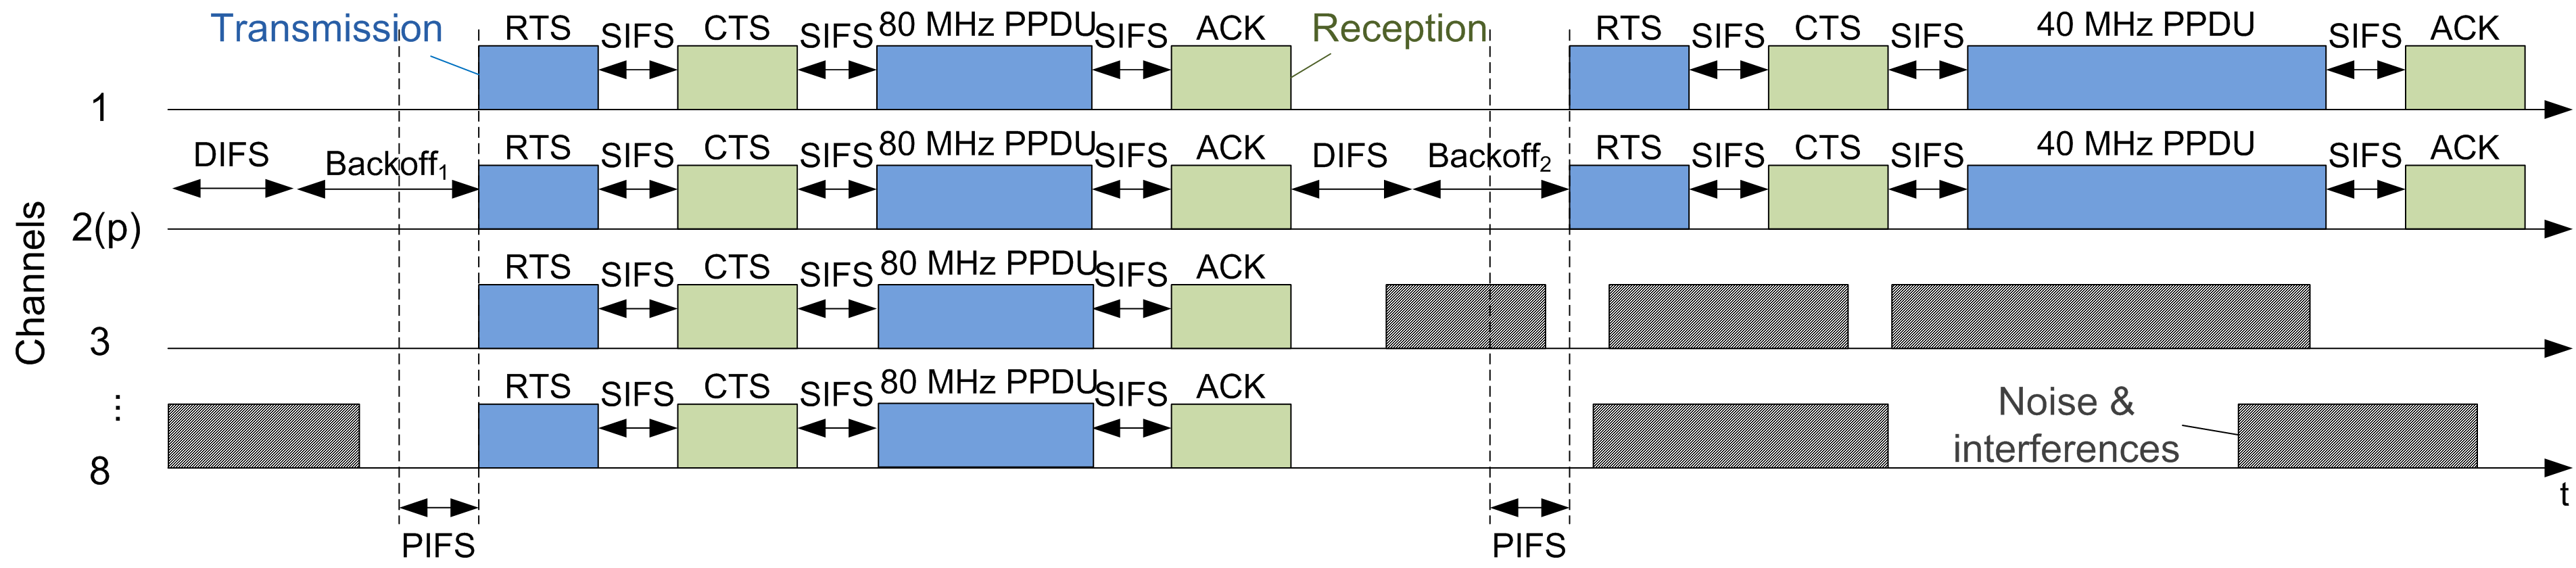
\includegraphics[width=0.95\textwidth]{images/dcb_dcf.png}
			\caption{CSMA/CA temporal evolution of a node operating under AM and the IEEE 802.11ax channelization scheme.}
			\label{fig:dcb_dcf}
		\end{figure}
		\item \textbf{Probabilistic uniform (PU)}: picks with same probability any of the possible channels found free inside the allocated channel.

	\end{itemize}

	For the sake of illustration, let us consider the example shown in Figure \ref{fig:dcb_dcf}, where the evolution of a node implementing AM is presented. Regarding the rest of DCB policies, \textit{i}) OP would just pick channel 2 after both backoff terminations, \textit{ii}) SCB would only transmit after the first backoff termination as part of the rest of basic channels is busy after the second one, and \textit{iii}) PU would transmit on channels $\{2\}, \{1,2\}, \{1,2,3,4\}$ or $\{1,2,...,8\}$ with same probability (1/4) at the first backoff termination, and on channels $\{2\}$ or $\{1,2\}$ with probability 1/2 at the end of the second one. An schematic flowchart of the DCB policy operation is shown in Figure \ref{fig:cb_policy_flowchart}.
	
	\begin{figure}[h]
		\centering
		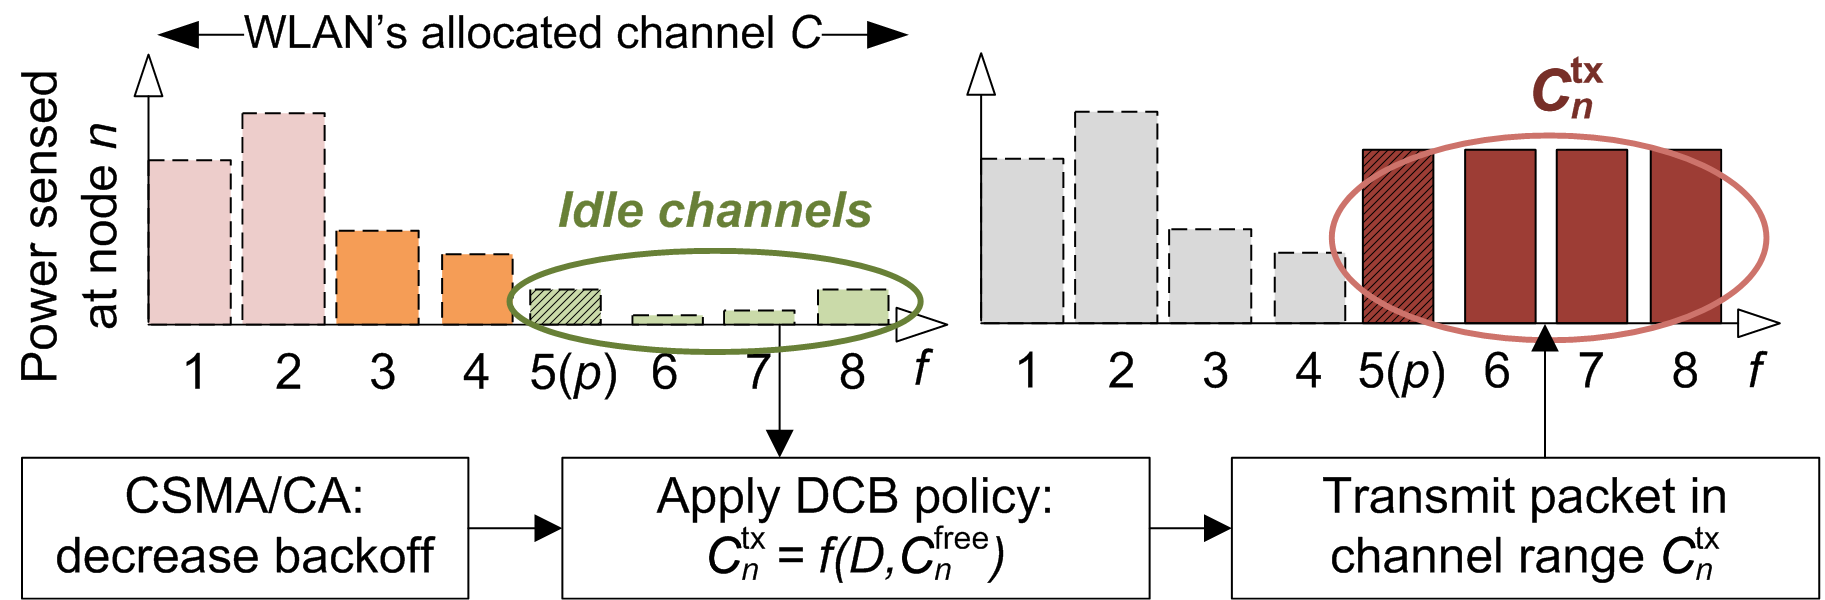
\includegraphics[width=0.64\textwidth]{images/cb_policy_flowchart.png}
		\caption{Flowchart of the transmission channel selection. In this example channel 5 is the primary channel and AM is applied.}    
		\label{fig:cb_policy_flowchart}
	\end{figure}
	

	%%% Packet Aggregation
	\subsection{Packet Aggregation}
	Packet aggregation aims to reduce transmission overheads such as headers, SIFS and DIFS intervals or backoff periods. For that, it concatenates $N$ MPDUs to be sent over the same packet transmission, so that it can be acknowledged through a block ACK. Komondor allows to define the number of aggregated packets, which value remains static during the entire simulation.
	\begin{figure}[h!]
		\centering
		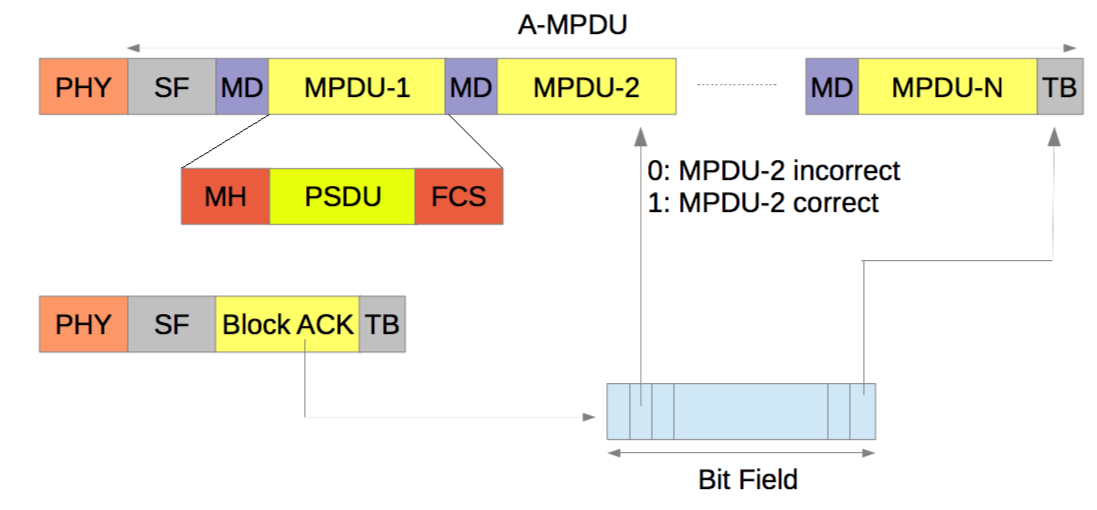
\epsfig{file=images/ampdu, width=10cm}
		\caption{Example of packet aggregation in which N MPDUs are concatenated to be sent during the same packet transmission.}
		\label{fig:ampdu}
	\end{figure}
	
%%%%%%%%%%%%%%%%
%% PHY FEATURES
%%%%%%%%%%%%%%%%
%\section{PHY Features}
%\label{section:phy_features}
%Similarly to previous Section, now we describe the PHY mechanisms implemented in Komondor.

%%%%%%%%%%%%%%%
% VALIDATIONS
%%%%%%%%%%%%%%%
\section{Komondor Main Features Validation through CTMN}
\label{section:validations}
	In this Section we aim to provide a mutual validate the core operation of Komondor by using a set of key scenarios. Moreover, we a mutual validation is done by considering the Continuous Time Markov Networks (CTMNs) model \cite{bellalta2014throughput}. To do so, we use the Spatial-Flexible Continuous Time Markov Network (SFCTMN),\footnote{All of the source code of SFCTMN is open, encouraging sharing of algorithms between contributors and providing the ability for people to improve on the work of others under the GNU General Public License v3.0. The code version used in this work can be found at \url{https://github.com/sergiobarra/SFCTMN}.} an analytical framework based on Continuous Time Markov Networks (CTMNs). This framework is useful for describing the different phenomena that occur in WLANs scenarios when considering DCB in non-spatially-constrained deployments, i.e., where nodes are not required to be within the carrier sense range of each other.

	%%% Parameters
	\subsection{IEEE 802.11ax Parameters}
	\label{section:parameters}
	Before showing the set of Komondor validations, we introduce in Table \ref{table:appendix_table} the IEEE 802.11ax parameters that we consider for simulations, and which are recommended to be kept in order to emulate 11ax's behavior.	
	
	\begin{table}[h]
		\caption{Parameters considered in the IEEE 802.11ax scenarios.}
		\label{table:appendix_table}
		\centering
		\begin{tabularx}{.8\textwidth}{vbv}
			\toprule
			
			\textbf{Parameter}     & \textbf{Description}              & \textbf{Value} \\ 
			
			\midrule
			
			$\text{CW}_\text{min}$ & Min. contention window            & 16             \\ 
			$m$                    & Backoff stage                     & 5              \\ 
			CCA                    & CCA threshold                               & -82 dBm        \\ 
			$P_\text{tx}$          & Transmission power                & 15 dBm         \\ 
			$G_\text{tx}$         & Transmitting gain                 & 0 dB           \\ 
			$G_\text{rx}$         & Reception gain                    & 0 dB           \\ 
			$L_\text{data}$       & Length of a data packet           & 12000 bits     \\ 
			$L_\text{BACK}$       & Length of a block ACK             & 240 bits       \\ 
			$L_\text{RTS}$        & Length of an RTS packet           & 160 bits       \\ 
			$L_\text{CTS}$        & Length of a CTS packet            & 112 bits       \\ 
			$n_\text{agg}$       & Num. data packets aggregated & 64             \\ 
			CE                     & Capture effect threshold          & 20 dB          \\ 
			$N$                      & Background noise level            & -95 dBm        \\ 
			$T_\text{slot}$       & Slot duration                     & 9 $\mu$s          \\ 
			SIFS                   & SIFS duration                     & 16 $\mu$s          \\ 
			DIFS                   & DIFS duration                     & 34 $\mu$s          \\ 
			PIFS                   & PIFS duration                     & 25 $\mu$s         \\ 
			$\eta$                 & Packet error rate        & 0.1           \\ 
			$f_c$                 & Central frequency       & 5 GHz           \\ 
			
			% IEEE 802.11ax
			$T_\text{ofdm}$      & OFDM symbol duration     & 16 $\mu$s           \\ 
			$T_\text{phy}$      & Legacy PHY header duration      & 20 $\mu$s           \\ 
			$n_\text{ss}$               & SU spatial streams       & 1           \\ 
			$T_\text{phy}^\text{HE}$      & HE header duration       & 32 $\mu$s \\ % $(16 + n_\text{ss} \cdot 16)$ $\mu$s           \\ 
			$L_\text{sfF}$      & Length of MAC's service field       & 16 bits           \\ 
			$L_\text{del}$      & Length of MAC's MPDU delimiter       & 32 bits           \\ 
			$L_\text{mac}$      & Length of MAC header     & 272 bits           \\ 
			$L_\text{tail}$      & Length of MAC's tail     & 6 bits           \\ 
			
			\bottomrule
		\end{tabularx}
	\end{table}

	%%% Basic Scenarios
	\subsection{Basic Operation Validation}
	\label{section:validations_basic_scenario}
%	Through the following scenarios, we aim to validate the basic operation of Komondor, so that features such as DCF and RTS/CTS can be properly tested.	The first validation we aim to show is at a very basic scenario in which two overlapping WLANs transmit by using $a)$ the same primary channel, $b)$ different non-overlapping channels. Such scenario is depicted in Figure \ref{fig:basic_scenario_1}. Furthermore, and in order to provide a more complete validation, we test Komondor's operation in the scenario shown in Figure \ref{fig:basic_scenario_2}. The four overlapping WLANs in such scenario are intended to use $a)$ the same primary channel, $b)$ two different channels, and $c)$ four different channels. 
%	\begin{figure}[h!]
%	\centering
% 	\begin{subfigure}[b]{0.475\textwidth}
%		\begin{tikzpicture}
%			\node at (0,0) [circle, fill=blue, draw, minimum width=0.5cm,minimum height=0.5cm, label=below:$\text{WLAN}_A$] (S1) {};
%			\node at (S1) [circle,draw=blue, minimum size=5cm, dashed] (S1c) {};
%			\node[circle, fill=red, draw, minimum width=0.5cm,minimum height=0.5cm, label=below:$\text{WLAN}_B$] (S2) [right of=S1, xshift=0.5cm] {};
%			\node at (S2) [circle,draw=red, minimum size=5cm, dashed] (S2c) {};
%		\end{tikzpicture}
%		\caption{Basic scenario 1} 
%		\label{fig:basic_scenario_1}
%	\end{subfigure}
%	\begin{subfigure}[b]{0.475\textwidth}
%		\begin{tikzpicture}
%		\node at (0,0) [circle, fill=green, draw, minimum width=0.5cm,minimum height=0.5cm, label=below:$\text{WLAN}_C$] (S1) {};
%		\node at (S1) [circle,draw=green, minimum size=5cm, dashed] (S1c) {};
%		\node[circle, fill=orange, draw, minimum width=0.5cm,minimum height=0.5cm, label=below:$\text{WLAN}_D$] (S2) [right of=S1, xshift=0.5cm] {};
%		\node at (S2) [circle,draw=orange, minimum size=5cm, dashed] (S2c) {};
%		\node[circle,draw, fill=blue, minimum width=0.5cm,minimum height=0.5cm, label=above:$\text{WLAN}_A$] (S3) [above of=S1, yshift=0.5cm] {};
%		\node at (S3) [circle,draw=blue, minimum size=5cm, dashed] (S3c) {};
%		\node[circle,draw, fill=red, minimum width=0.5cm,minimum height=0.5cm, label=above:$\text{WLAN}_B$] (S4) [above of=S2, yshift=0.5cm] {};
%		\node at (S4) [circle,draw=red, minimum size=5cm, dashed] (S4c) {};	
%		\end{tikzpicture}
%		\caption{Basic scenario 2}
%		\label{fig:basic_scenario_2}
%	\end{subfigure}
%	\caption{Scenarios for basic validations}
%	\label{fig:basic_scenario}
%	\end{figure}
%
%	Results from simulation in each of the basic scenarios are presented in Table \ref{table:basic_scenarios}.
%	\begin{table}[h!]
%		\centering
%		\begin{tabular}{|c|c|c|c|c|c|c|}
%			\hline
%			\textbf{Scenario} & \textbf{Tool} & $\Gamma_A$ & $\Gamma_B$ & $\Gamma_C$ & $\Gamma_D$ & $\Gamma$ \\ \hline
%			\multirow{2}{*}{1a} & Komondor & 51.17 & 51.12 & - & - & 102.29 \\ \cline{2-7} 
%			& CTMN & 66.71 & 66.71 & - & - & 133.42 \\ \hline
%			\multirow{2}{*}{1b} & Komondor & 101.66  & 101.71 & - & - & 203.37 \\ \cline{2-7} 
%			& CTMN & 132.81 & 132.81 & - & - & 265.63 \\ \hline
%			\multirow{2}{*}{2a} & Komondor & 12.45 & 12.50 & 12.47 & 12.49 & 49.91 \\ \cline{2-7} 
%			& CTMN & 33.43 & 33.43 & 33.43 & 33.43 & 133.72 \\ \hline
%			\multirow{2}{*}{2b} & Komondor & 50.99 & 50.97 & 51 & 51.02 & 203.98 \\ \cline{2-7} 
%			& CTMN & 66.71 & 66.71 & 66.71 & 66.71 & 266.84 \\ \hline
%			\multirow{2}{*}{2c} & Komondor & 101.19 & 101.23 & 101.18 & 101.19 & 404.78 \\ \cline{2-7} 
%			& CTMN & 132.81 & 132.81 & 132.81 & 132.81 & 531.24 \\ \hline
%		\end{tabular}
%		\caption{Summary of the results obtained for the basic scenarios.}
%		\label{table:basic_scenarios}
%	\end{table}	
		
	The basic operation of Komondor regarding the DCF implementation with additional features such as RTS/CTS is first validated in the scenario shown in Figure \ref{fig:basic_scenario}, which frames a single WLAN composed by an AP and two STAs. All the devices are within the same range, so that channel access is completely fair. However, in order to give priority to the AP, its CW is smaller than the one used by STAs. The performance achieved by each device is shown in \ref{table:basic_scenario_results}, where Komondor results are compared to equivalent ns-3 simulations, and to the Bianchi's analytical model \cite{bianchi2000performance}. 
	
	\begin{figure}[h!]
		\centering
		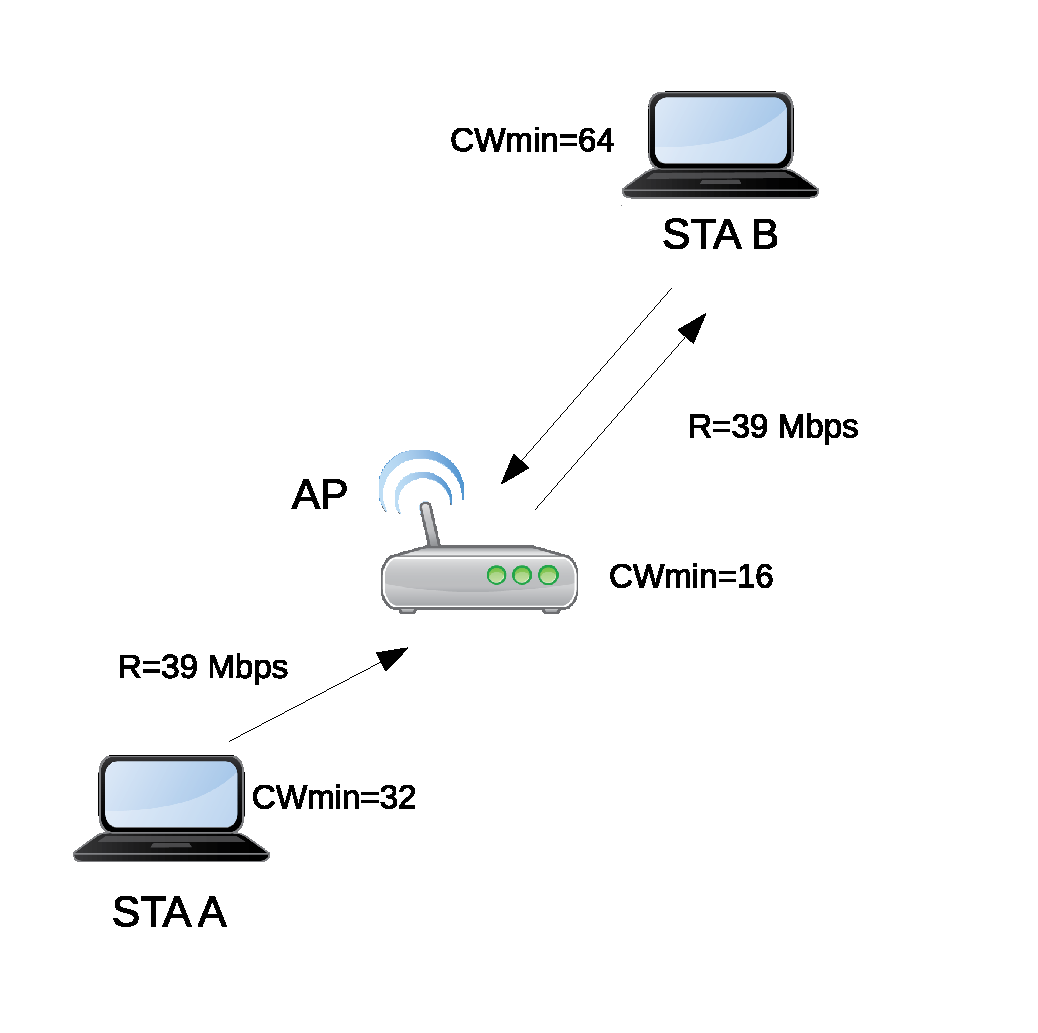
\epsfig{file=images/Seminar3_2.eps, width=7cm}
		\caption{SCENARIO I (TEMPORARY IMAGE)}
		\label{fig:basic_scenario}
	\end{figure}	
	
	\begin{table}[h!]
		\centering
		\caption{Results for Komondor validations in Scenario I. The average throughput experienced by each device is shown for ns-3, Bianchi and CTMNs simulations.}
		\label{table:basic_scenario_results}
		\begin{tabular}{|l|c|c|c|c|}
			\hline
			& Komondor & ns-3 & Bianchi & CTMNs \\ \hline
			$\Gamma_{AP}$ &  &  & & \\ \hline
			$\Gamma_{STA A}$ &  &  & & \\ \hline
			$\Gamma_{STA B}$ & \multicolumn{1}{l|}{} & \multicolumn{1}{l|}{} & \multicolumn{1}{l|}{} & \multicolumn{1}{l|}{} \\ \hline
		\end{tabular}
	\end{table}

	%%% Complex interactions Scenarios
	\subsection{Complex Interactions Validation}
	\label{section:validations_complex_scenario}
	
	Now, in order to further validate the Komondor simulator, we propose the following set of partial-overlapping scenarios, which are shown in Figure \ref{fig:scenario_III}:
	\begin{itemize}
		\item \textbf{Topology 1 (\emph{T1})}: all the nodes are able to listen each other, so that they share the channel on equal terms.
		\item \textbf{Topology 2 (\emph{T2})}: either $\text{AP}_A$ or $\text{AP}_C$ generate enough interference to contend $\text{AP}_B$'s transmission.
		\item \textbf{Topology 3 (\emph{T3})}: simultaneous transmission of both $\text{AP}_A$ and $\text{AP}_C$ generates enough interference to make $\text{AP}_B$ sense the channel busy.
		\item \textbf{Topology 4 (\emph{T4})}: none of the nodes' transmission is sensed by the others.
	\end{itemize}
	
	\begin{figure*}
		\centering
		\begin{subfigure}{.5\textwidth}
			\centering
			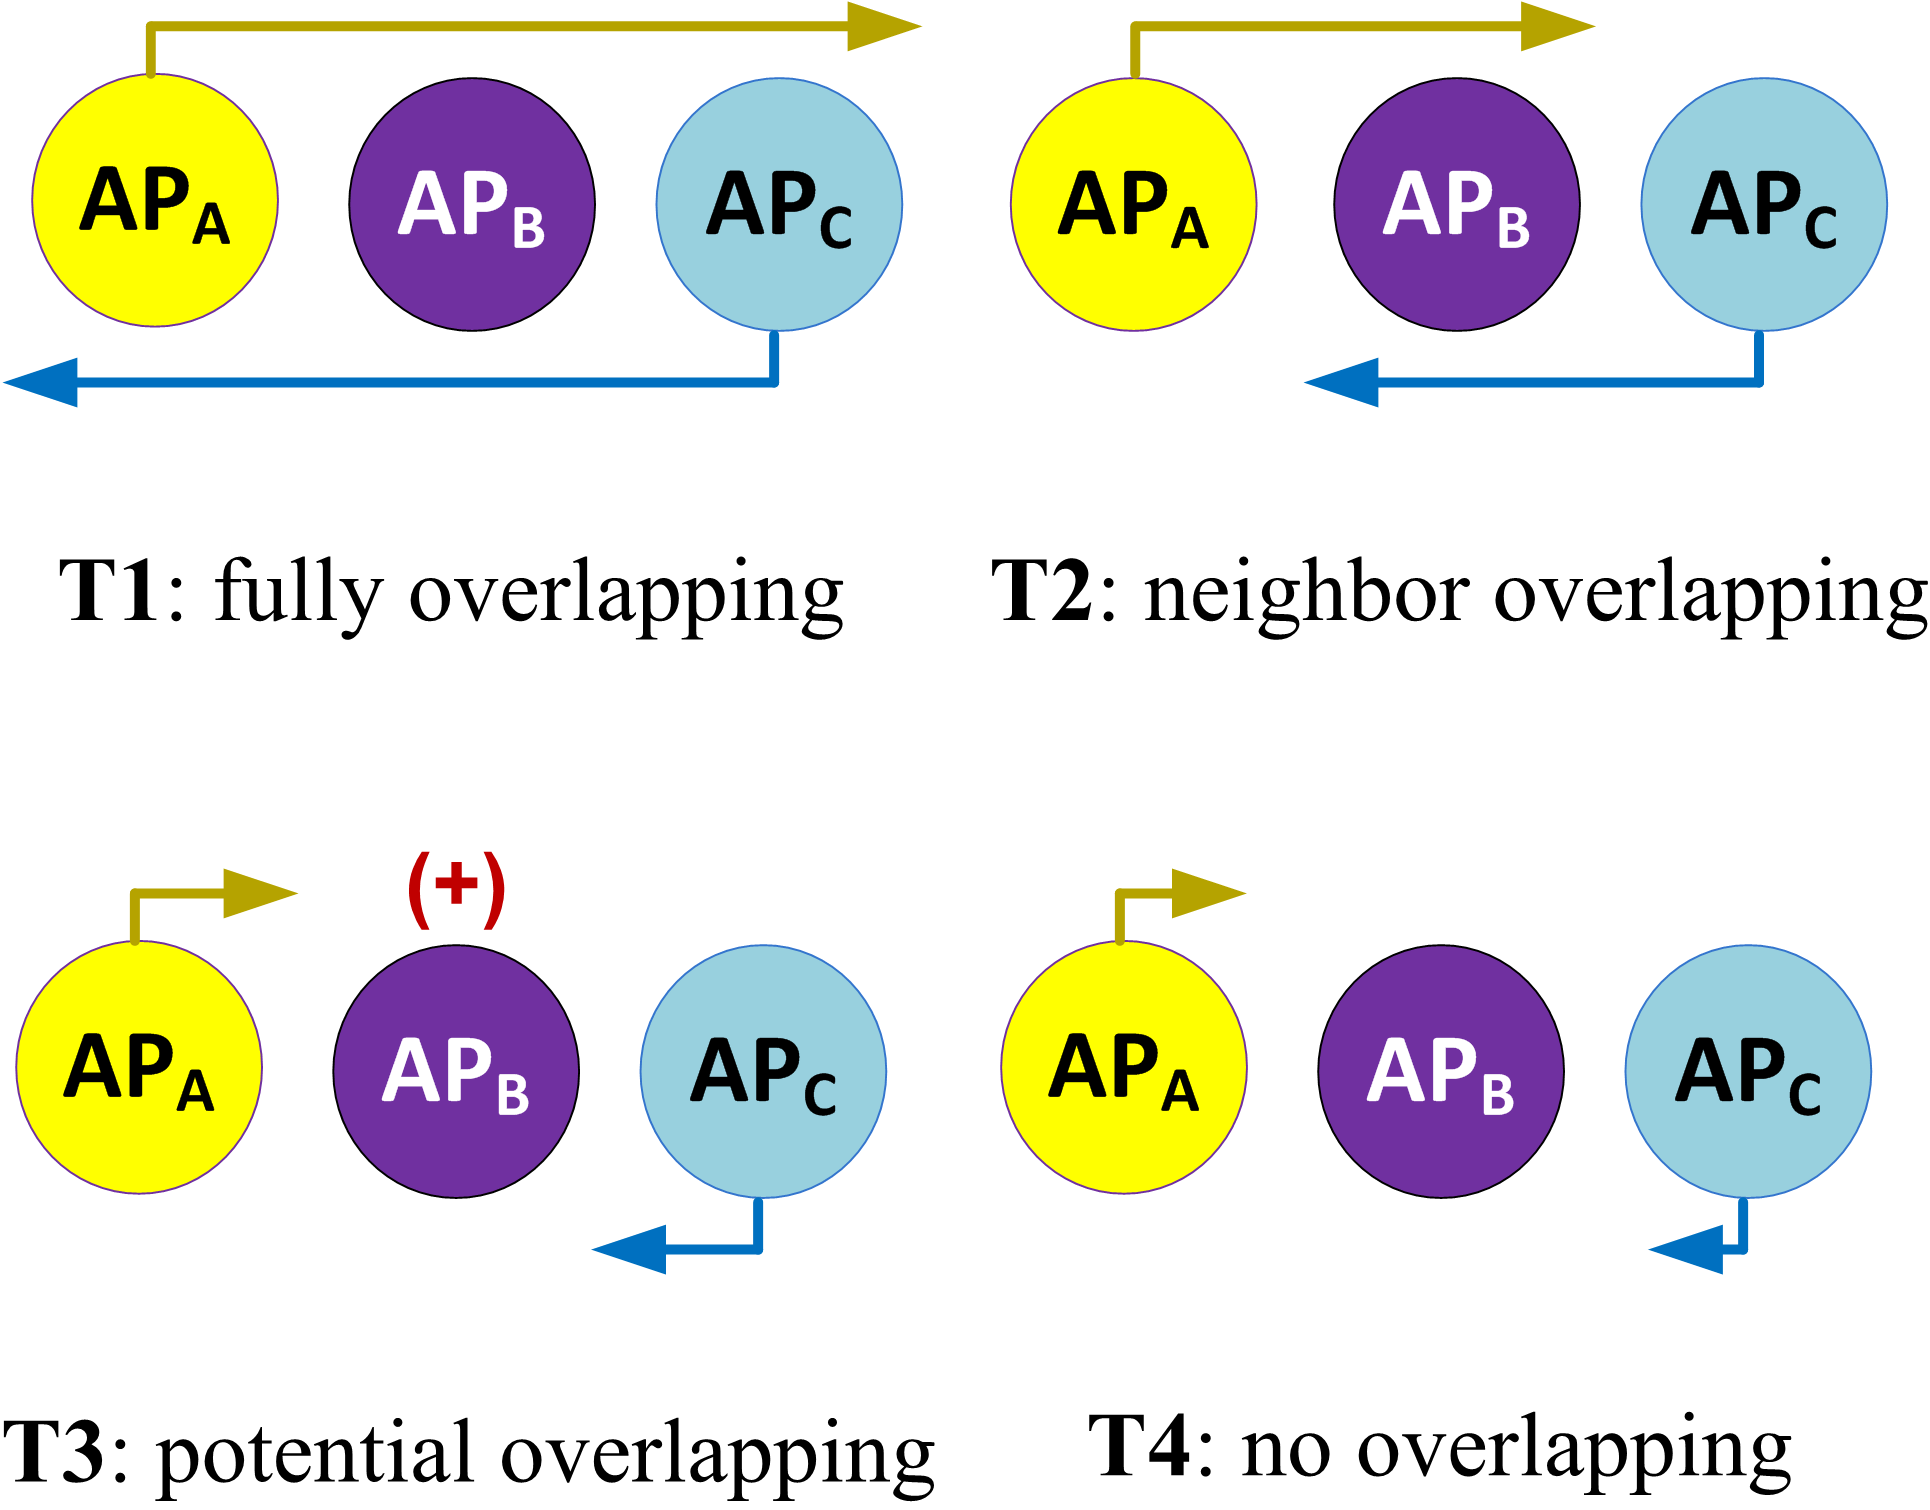
\includegraphics[width=.75\linewidth]{images/scenario_III.png}
			\caption{Topologies}
			\label{fig:scenario_III}
		\end{subfigure}%
		\begin{subfigure}{.5\textwidth}
			\centering
			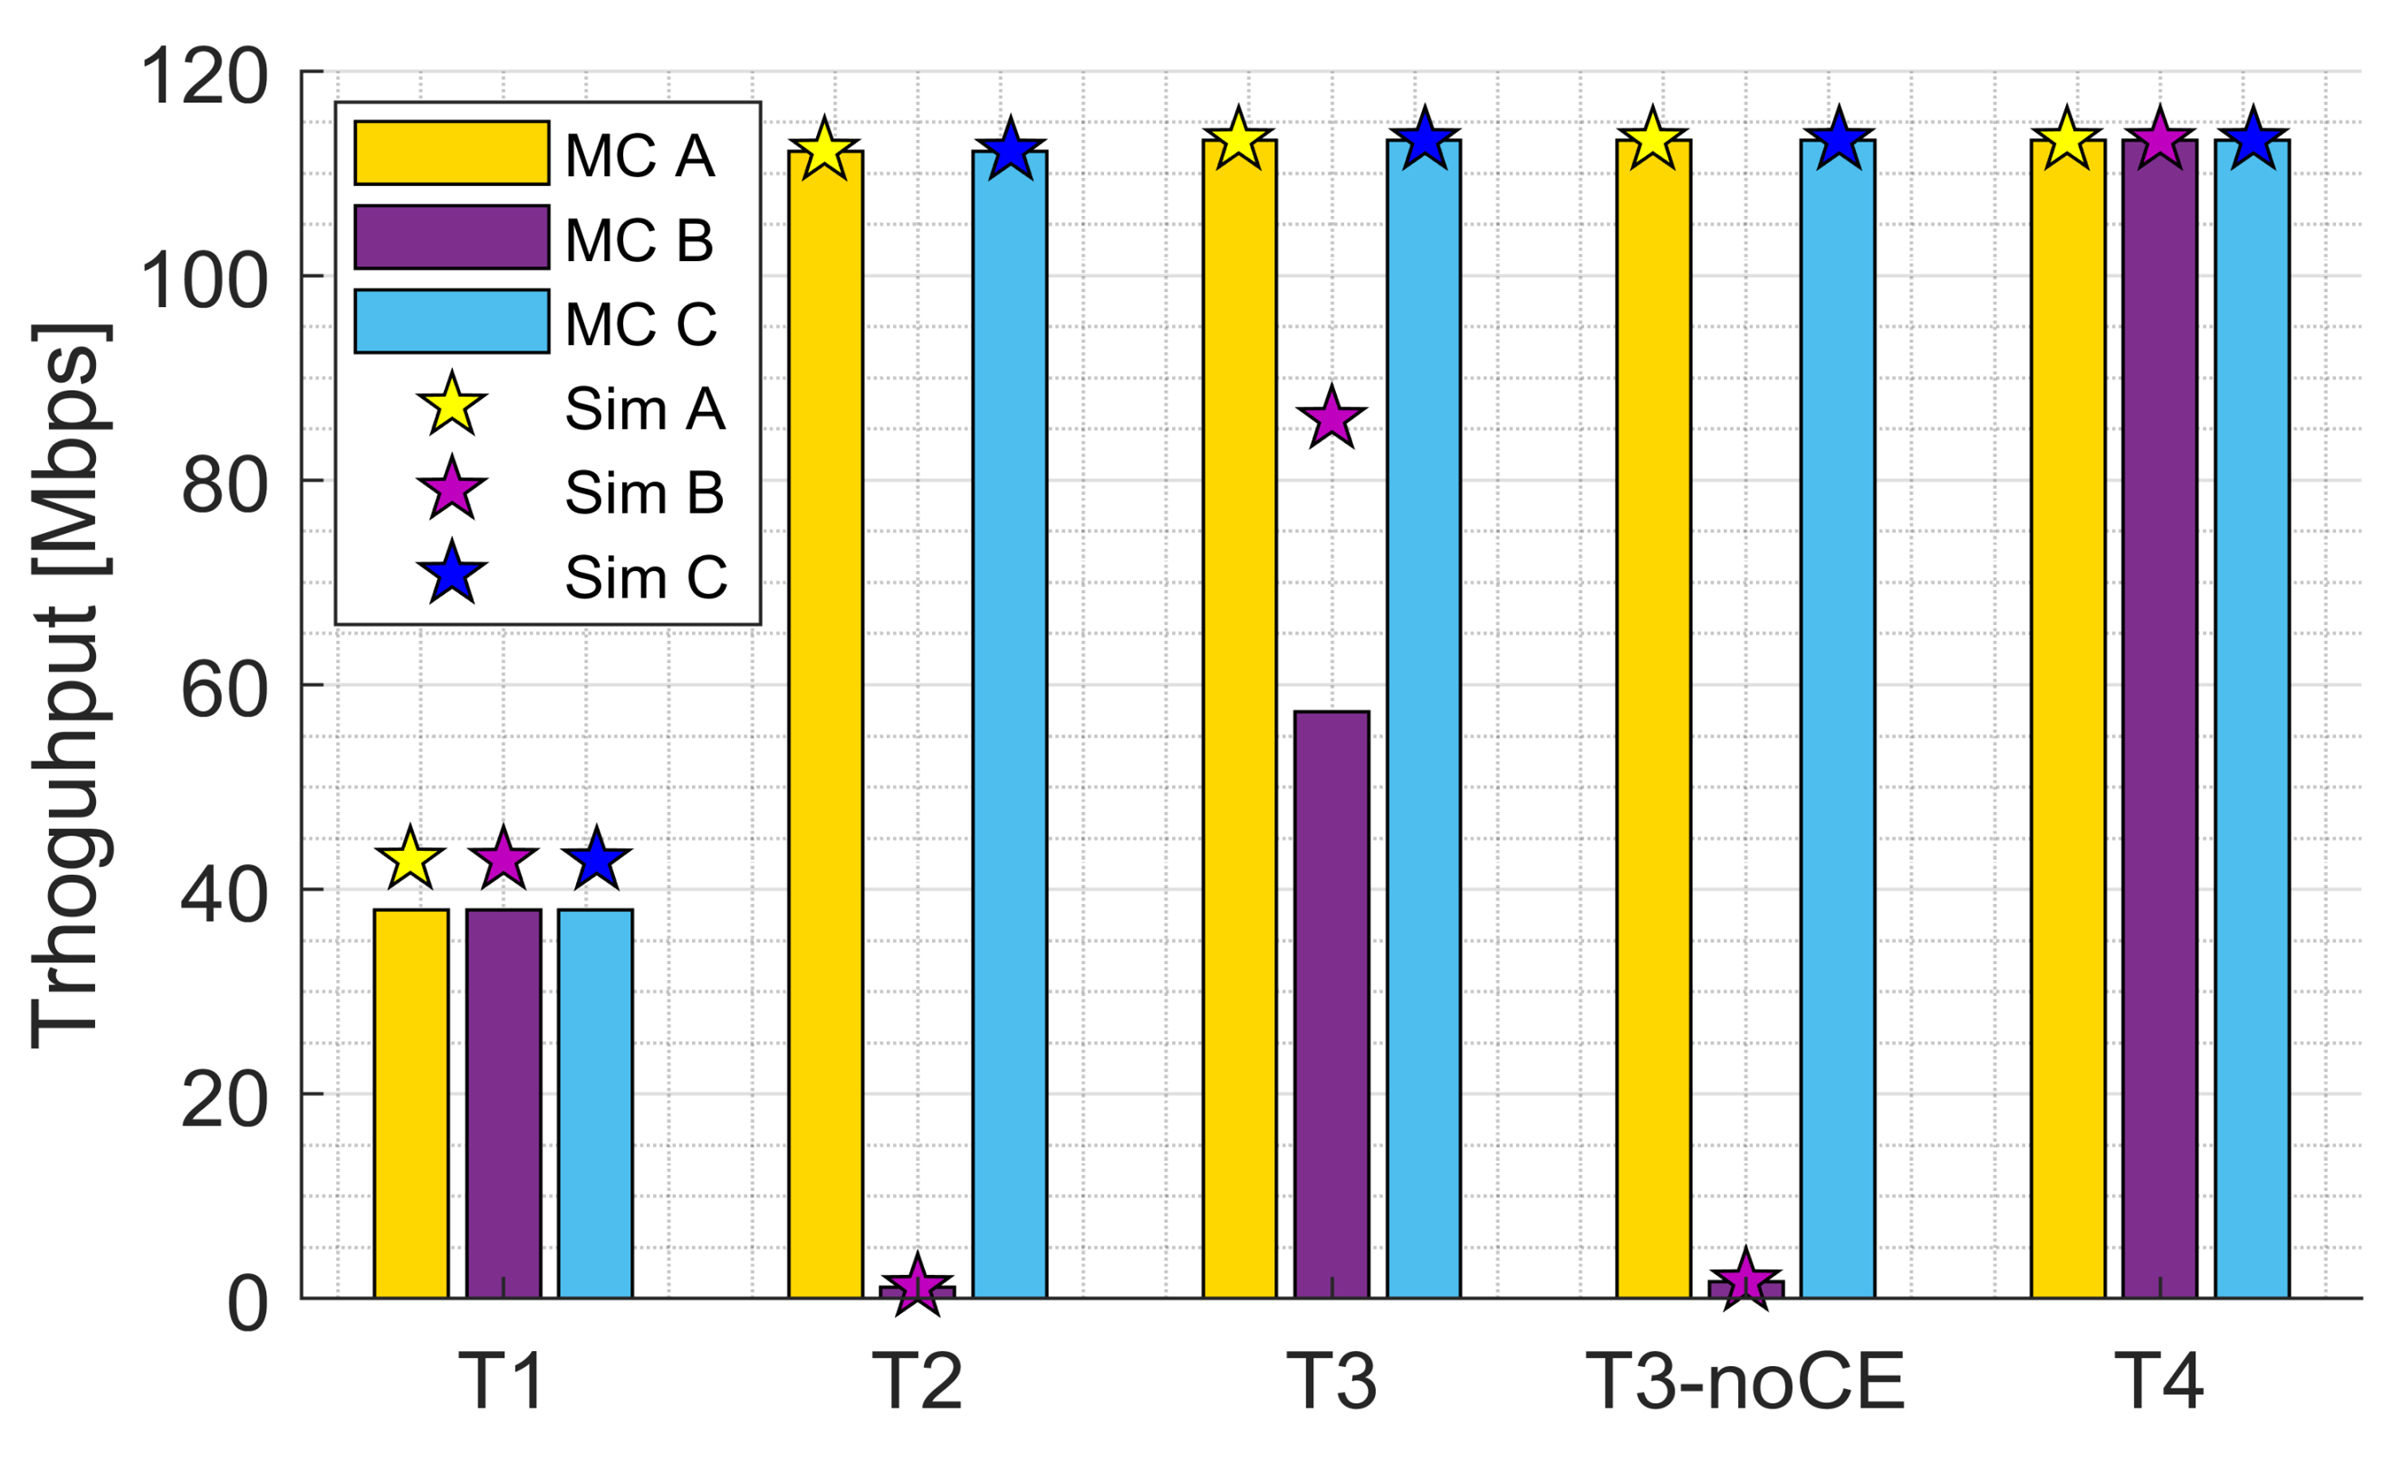
\includegraphics[width=0.95\linewidth]{images/scenario3_results_sfctmn_komondor.png}
			\caption{Average throughput}
			\label{fig:scenario3_results_sfctmn_komondor}
		\end{subfigure}
		\caption{Scenarios and results for Komondor validations. Yellow and blue arrows indicate the carrier sense range of WLANs A and C, respectively (CST is equal for all the APs). The carrier sense range of WLAN B is not displayed. \textit{T3-noCE} refers to topology \textit{T3} when the STA in B does not accomplish the CE condition whenever A, B and C are active. MC and Sim refer to the values obtained through SFCTMN and Komondor, respectively.}
		\label{fig:scenario_III_all}
	\end{figure*}
	
	% Results full overlapping T1
	The average throughput experienced by each WLAN in each of the regions is shown in Figure \ref{fig:scenario3_results_sfctmn_komondor}. Regarding topology \textit{T1}, when APs are close enough to be inside the carrier sense range of each other in a fully-overlapping manner, the medium access is shared fairly because of the CSMA/CA mechanism. For that reason, the throughput is decreased to approximately 1/3 with respect to topology \textit{T4}. Regarding the difference between Komondor and CTMNs results, note that successful simultaneous transmissions (or slotted backoff collisions) are allowed in Komondor, as well as the capture effect is accomplished. Henceforth, the throughput is slightly higher in Komondor.
	
	% Results neighbor overlapping T2
	The neighbor overlapping case in topology \textit{T2}, where A and C can transmit at the same time whenever B is not active, but B can only do so when both A and C are not active, is a clear case of exposed-node starvation. Namely, B has very few transmission opportunities as A and C are transmitting almost permanently and B must continuously freeze its backoff consequently. 
	
	% Results potential central node overlapping T3
	Regarding \textit{T3}, the sum of the interference that B perceives when A and C are transmitting at the same time prevents it to decrease the backoff. However, B is able to decrement the backoff any time A or C are not transmitting.
	
	% Results isolation T4
	Finally, in topology \textit{T4}, due to the fact that WLANs are isolated, the number of successful parallel transmissions is maximum.
	
%	%%% Hidden and Exposed Scenarios
%	\subsection{Hidden and Exposed Node Scenarios}
%	\label{section:validations_hidden_exposed}
%	We start showing a hidden-node situation in which two simultaneously transmit to the their respective STAs, as shown in Figure \ref{fig:hidden_node_scenario}. Due to nodes location, transmitters (i.e., the APs) do not sense each other, so that they simultaneously transmit and generate collisions at the receivers (e.g., the STAs), which are in the middle. 
%	
%	Regarding the exposed node situation, we introduce the scenario depicted in Figure \ref{fig:exposed_node_scenario}, in which one of the three WLANs suffers starvation because of its location. The fact that $\text{WLAN}_A$ and $\text{WLAN}_C$ do not sense each other makes that $\text{WLAN}_B$ senses the channel busy almost all the time and lacks of opportunities for accessing to it.
%	\begin{figure}[h!]
%	\centering
%	\begin{subfigure}[b]{0.5\textwidth}
%		\begin{tikzpicture}
%		\node at (0,0) [circle, fill=red, draw, minimum width=0.5cm,minimum height=0.5cm, label=below:$\text{AP}_A$] (A) {};
%		\node at (A) [circle,draw=red, minimum size=4.5cm, dashed] (Ac) {};
%		\node[circle, fill=red, draw, minimum width=0.5cm,minimum height=0.5cm, label=below:$\text{STA}_A$] (B) [right of=A, xshift=0.1cm] {};
%		%\node at (B) [circle,draw=red, minimum size=3.5cm, dashed] (Bc) {};
%		\node[circle,draw, fill=blue, minimum width=0.5cm,minimum height=0.5cm, label=below:$\text{STA}_B$] (C) [right of=B, xshift=0.01cm] {};
%		%\node at (C) [circle,draw=blue, minimum size=3.5cm, dashed] (Cc) {};      
%		\node[circle,draw, fill=blue, minimum width=0.5cm,minimum height=0.5cm, label=below:$\text{AP}_B$] (D) [right of=C, xshift=0.1cm] {};
%		\node at (D) [circle,draw=blue, minimum size=4.5cm, dashed] (Cc) {};
%		\draw [->,line width=1.8pt] (A) edge (B) (D) edge (C);
%		\end{tikzpicture}
%		\caption{Hidden-node} 
%		\label{fig:hidden_node_scenario}
%	\end{subfigure}
%	\begin{subfigure}[b]{0.5\textwidth}
%		\begin{tikzpicture}
%		\node at (0,0) [circle, fill=red, draw, minimum width=0.5cm,minimum height=0.5cm, label=below:$\text{WLAN}_A$] (A) {};
%		\node at (A) [circle,draw=red, minimum size=4cm, dashed] (Ac) {};
%		\node[circle, fill=orange, draw, minimum width=0.5cm,minimum height=0.5cm, label=below:$\text{WLAN}_B$] (B) [right of=A, xshift=0.5cm] {};
%		\node at (B) [circle,draw=orange, minimum size=4cm, dashed] (Bc) {};
%		\node[circle,draw, fill=blue, minimum width=0.5cm,minimum height=0.5cm, label=below:$\text{WLAN}_C$] (C) [right of=B, xshift=0.5cm] {};
%		\node at (C) [circle,draw=blue, minimum size=4cm, dashed] (Cc) {};      
%		\end{tikzpicture}
%		\caption{Exposed-node}
%		\label{fig:exposed_node_scenario}
%	\end{subfigure}
%	\caption{Representative scenarios of performance anomalies in WLANs} 
%	\label{fig:anomalies_scenario}
%	\end{figure}
%
%	Results for both hidden and exposed scenarios are shown in Table \ref{table:hidden_exposed_scenarios}.
%	% Please add the following required packages to your document preamble:
%	% \usepackage{multirow}
%	\begin{table}[]
%		\centering
%		\begin{tabular}{|c|c|c|c|c|c|c|}
%			\hline
%			\textbf{Scenario} & \textbf{Tool} & $\Gamma_A$ & $\Gamma_B$ & $\Gamma_C$ & $\Gamma$ & Loss rate \\ \hline
%			\multirow{2}{*}{\begin{tabular}[c]{@{}c@{}}Hidden\\ node\end{tabular}} & Komondor & 0 & 0 & - & 0 & 1  \\ \cline{2-7} 
%			& CTMN & 0 & 0 & - & 0 & 1 \\ \hline
%			\multirow{2}{*}{\begin{tabular}[c]{@{}c@{}}Exposed\\ node\end{tabular}} & Komondor & 101.07 & 0.64 & 101.07 & 202.77 & 0.11* \\ \cline{2-7} 
%			& CTMN & 131.64 & 1.19 & 131.64 & 264.47 & 0 \\ \hline
%		\end{tabular}
%		\caption{Summary of the results obtained for the hidden and exposed node scenarios. *A constant packet loss rate of 0.1 is set to simulate losses when using an acceptable MCS.}
%		\label{table:hidden_exposed_scenarios}
%	\end{table}	

	%%% Channel Bonding Scenarios
	\subsection{Dynamic Channel Bonding Validation}
	\label{section:validations_channel_bonding}
	Finally, we validate one of the most important techniques included in the Komondor simulator, which is Dynamic Channel Bonding. In order to do that, we introduce the scenarios shown in Figure \ref{fig:cb_scenarios}, which consider two overlapping WLANs.
	% Scenario I figure
	\begin{figure}[h!]
		\centering
		\begin{subfigure}[b]{0.475\textwidth}
			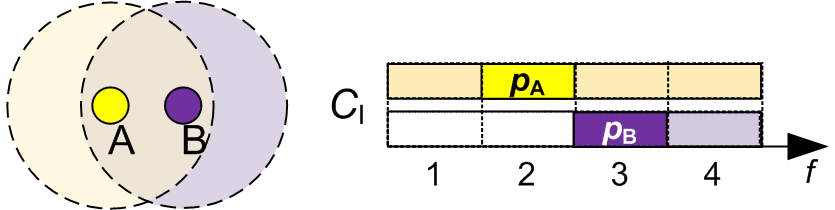
\includegraphics[width=1\textwidth]{images/scenario_I.png}
			\caption{\textit{Scenario I}}
			\label{fig:scenario_I}
		\end{subfigure}
		\begin{subfigure}[b]{0.475\textwidth}
			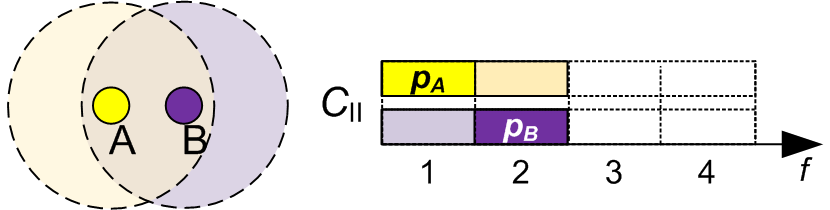
\includegraphics[width=1\textwidth]{images/scenario_II.png}
			\caption{\textit{Scenario II}}
			\label{fig:scenario_II}
		\end{subfigure}
		\caption{WLANs A and B are inside the carrier sense range of each other with potentially overlapping channels 1 and 2.}
		\label{fig:cb_scenarios}
	\end{figure}
	
	In Table \ref{table:cb_policy_effect} we show the results from applying the different DCB policies introduced in Section \ref{section:channel_bonding}. We display the average throughput experienced by WLANs A and B ($\Gamma_\text{A}$ and $\Gamma_\text{B}$, respectively), and by the whole network ($\Gamma$).
	\begin{table}[h]
		\centering
			\setlength\tabcolsep{1.5pt} % default value: 6pt
			\begin{tabular}{c|c|c|c|c|c|c|c|c|}
				\cline{2-9}
				& \multicolumn{4}{c|}{\textit{Scenario I}}                                  & \multicolumn{4}{c|}{\textit{Scenario II}}                                \\ \hline
				\multicolumn{1}{|c|}{$\mathcal{D}$}                    & $|\mathcal{S}|$              & $\Gamma_A$ & $\Gamma_B$ & $\Gamma$ & $|\mathcal{S}|$             & $\Gamma_A$ & $\Gamma_B$ & $\Gamma$ \\ \hline
				
				\multicolumn{1}{|c|}{\multirow{2}{*}{OP}}  & \multirow{2}{*}{4}  & 113.23     & 113.23     & 226.47   & \multirow{2}{*}{4} & 113.23     & 113.23     & 226.47   \\  
				\multicolumn{1}{|c|}{}                     &                     & \textcolor{blue}{113.23}     & \textcolor{blue}{113.23}     & \textcolor{blue}{226.46}   &                    & \textcolor{blue}{113.23}     & \textcolor{blue}{113.23}     & \textcolor{blue}{226.46}   \\ \hline
				
				\multicolumn{1}{|c|}{\multirow{2}{*}{SCB}} & \multirow{2}{*}{3}  & 143.46     & 143.46     & 286.92   & \multirow{2}{*}{3} & 109.19     & 109.19     & 218.38   \\
				\multicolumn{1}{|c|}{}                     &                     & \textcolor{blue}{131.98}     & \textcolor{blue}{148.85}     & \textcolor{blue}{280.83}   &                    & \textcolor{blue}{108.72}     & \textcolor{blue}{108.84}     & \textcolor{blue}{217.56}   \\ \hline
	
				\multicolumn{1}{|c|}{\multirow{2}{*}{AM}}  & \multirow{2}{*}{5}  & 220.12     & 212.21     & 432.34   & \multirow{2}{*}{3} & 109.19     & 109.19     & 218.38   \\ 
				\multicolumn{1}{|c|}{}                     &                     & \textcolor{blue}{217.60}     & \textcolor{blue}{214.81}     & \textcolor{blue}{432.41}   &                    & \textcolor{blue}{108.72}     & \textcolor{blue}{108.84}     & \textcolor{blue}{217.56}   \\ \hline
				
				\multicolumn{1}{|c|}{\multirow{2}{*}{PU}}  & \multirow{2}{*}{10} & 149.14     & 148.38     & 297.52   & \multirow{2}{*}{6} & 113.19     & 113.19     & 226.38   \\  
				\multicolumn{1}{|c|}{}                     &                     & \textcolor{blue}{149.20}     & \textcolor{blue}{148.42}     & \textcolor{blue}{297.63}   &                    & \textcolor{blue}{113.20}     & \textcolor{blue}{113.18}     & \textcolor{blue}{226.38}   \\ \hline
			\end{tabular}
		\caption{DCB policy effect on the average throughput [Mbps] in \textit{Scenario I} and \textit{Scenario II}. The values obtained through Komondor are displayed in blue, while the other correspond to the CTMN model.}
		\label{table:cb_policy_effect}
	\end{table}

	% Explain CB policy effect on scenario I. DCB
	Let us first consider \textit{Scenario I}. As expected, due to the fact that both WLANs overlap in channels 3 and 4 when transmitting in their whole allocated channels, the SCB policy reaches just three feasible states in which WLANs cannot transmit at the same time. In the case of OP both WLANs are forced to pick just their primary channel for transmitting and, therefore, they can transmit simultaneously.	
	% Explain CB policy effect on scenario I. always-max
	Regarding the AM policy, which is usually used as de-facto when applying DCB, it allows simultaneous transmissions provided that WLAN B started transmitting when the channel was idle. Notice that with AM, any time the backoff of an AP in WLAN X expires and the channel is idle, a given AP would pick the the widest available channel. 	
	% Explain CB policy effect on scenario I. Prob. uniform
	The last policy studied is PU, which is characterized by providing further exploration regarding the possible channel range combinations. In scenario I, whenever the channel is idle and the backoff of either A or B expires, each of the possible available channel ranges may be chosen with same probability. For instance, A may choose channel ranges 2, 1-2 or 1-4 with probability 1/3. Similarly, B may choose transmitting over channels 3 or 3-4.
	
	Intuitively, one could think that, as it occurs in \textit{Scenario I}, picking always the widest channel found free by means of AM, i.e., maximizing the throughput of the immediate transmission (or short-term throughput), may be the best strategy for optimizing the long-term throughput as well. However, the \textit{Scenario II} depicted in Figure \ref{fig:scenario_II}, is a counterexample that illustrates such lack of applicable intuition. Firstly, with OP, due to the fact that WLANs are only allowed to transmit in their primary channel, simultaneous transmissions can be carried out. On the other hand, with SCB, WLANs can only transmit in their complete allocated channel, thus allowing a single transmission at a time. Notice that in this case AM generates the same transition probabilities (and respective average throughput) than SCB because whenever a WLAN has the possibility to transmit. Finally, PU picks uniformly at random any of the possible channel combinations that A and B may choose when terminating their backoff in case that the channel is idle.
			
	% Differences between SFCTM and Komondor I
	Concerning the throughput differences in the values obtained by CTMNs and Komondor, we note that the main disparities correspond to the AM and SCB policies. It is important to remark that while CTMN does not consider neither backoff collisions nor NAV periods, Komondor actually does so in a realistic way. Therefore, in Komondor, whenever there is a slotted backoff collision, the RTS packets can be decoded by the STAs in both WLANs and the average throughputs are increased consequently.	
	% Differences between SFCTM and Komondor II
	Regarding the NAV periods, an interesting phenomena occurs in \textit{Scenario I} when implementing SCB, AM or PU. While the RTS packets sent by B cannot be decoded by A because its primary channel is always outside the transmission channel range of B, the opposite occurs when A sends them. Due to the fact that the RTS is duplicated in each of the basic channels used for transmitting, whenever A transmits in its whole allocated channel, B is able to decode the RTS and enters in NAV consequently. 

%%%%%%%%%%%%%%%
% TUTORIAL
%%%%%%%%%%%%%%%
\section{Tutorial and Development Notes}
\label{section:tutorial_and_development_notes}
	In this Section we provide a brief tutorial to encourage researchers and other practitioners to use the Komondor simulator for their own experiments, and even to participate in the project. 
	%%% Brief tutorial
	\subsection{Brief Tutorial}
	\label{section:brief_tutorial}
		Komondor is composed by several modules that allow performing simulations with a high degree of freedom. Here we provide some details on the most important modules, as well as on their practical execution. Figure \ref{fig:komondor_flowchart} summarizes the main operations carried out by Komondor.
		\begin{figure}[h!]
			\centering
			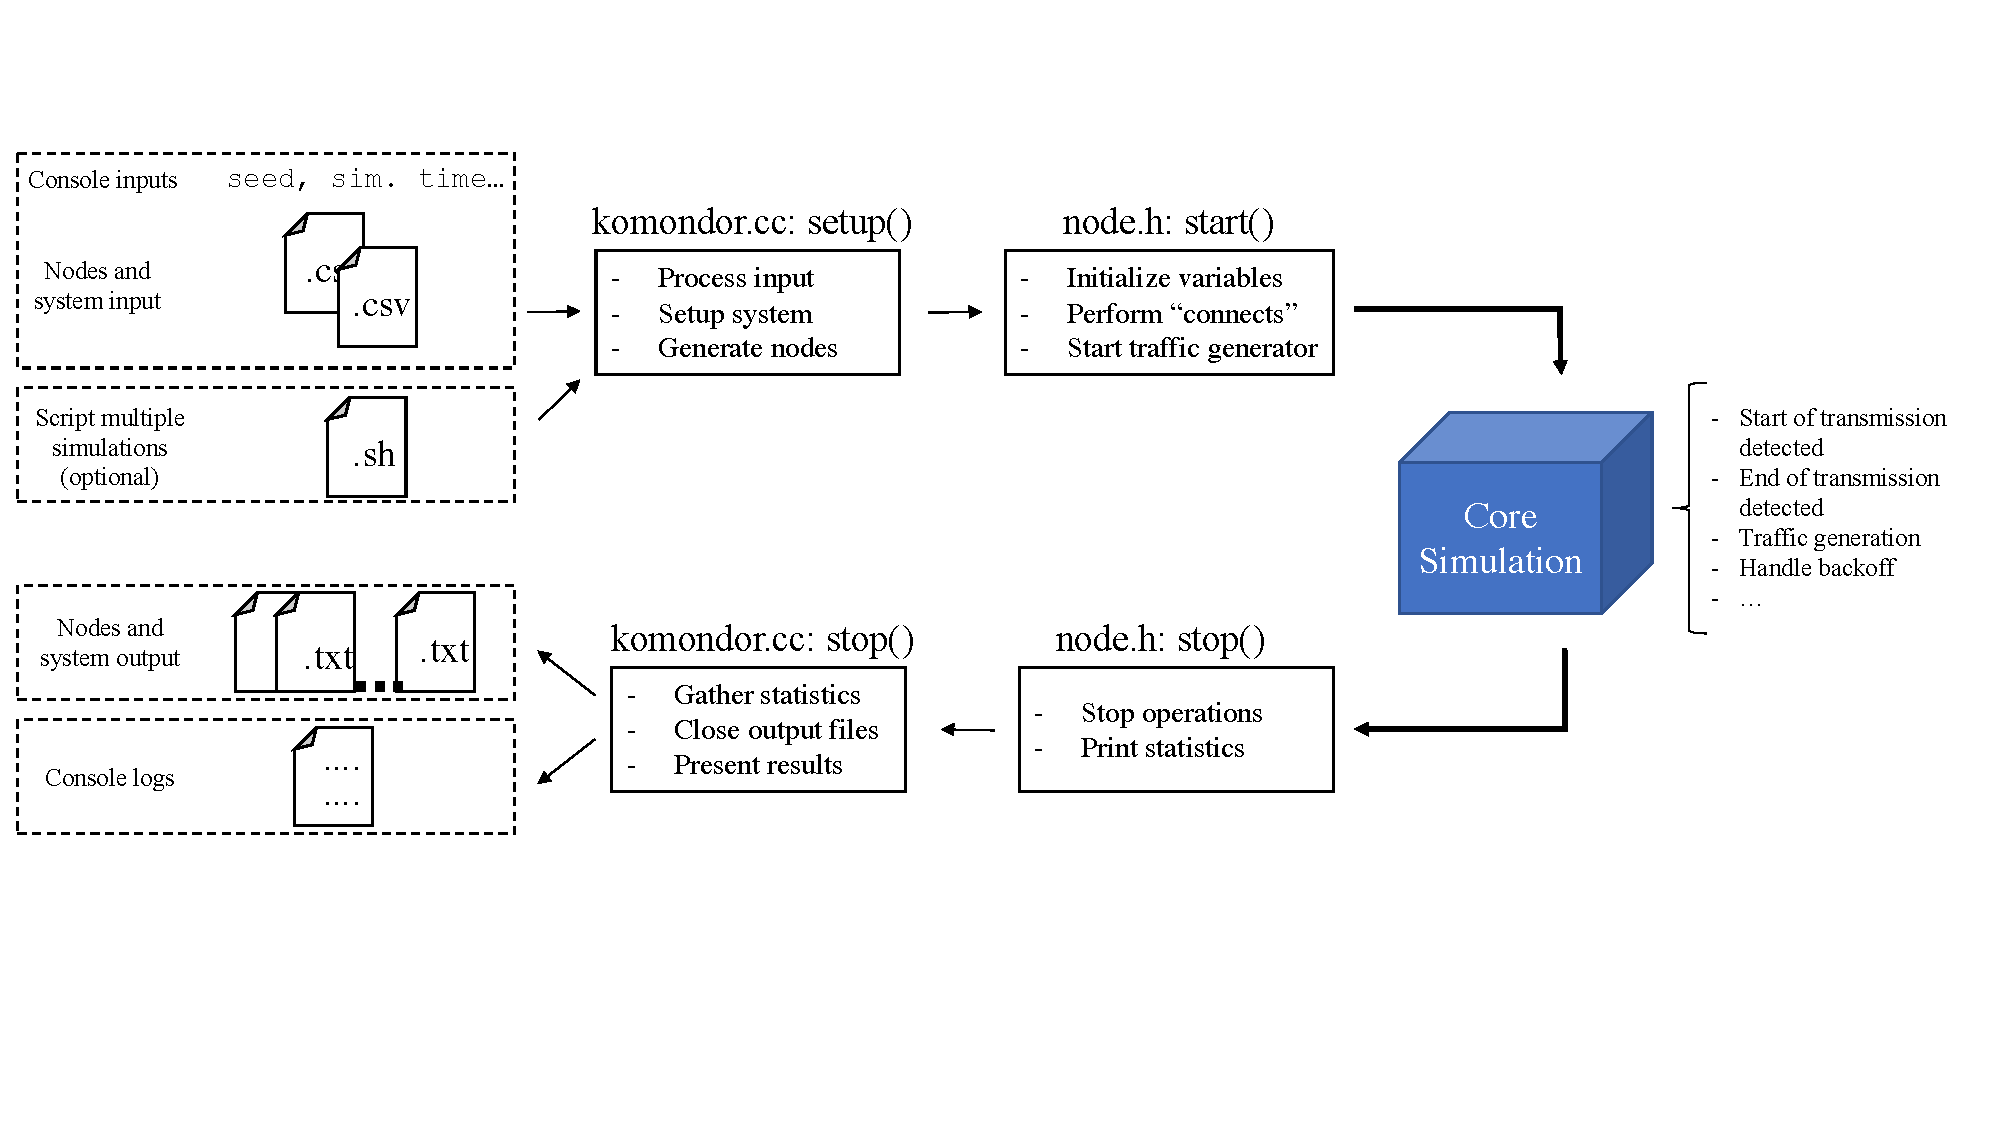
\epsfig{file=images/komondor_flowchart, width=15cm}
			\caption{Komondor flowchart}
			\label{fig:komondor_flowchart}
		\end{figure}		
		
		As shown, Komondor receives a set of inputs (nodes information, simulation time, etc.) and initializes the main module, which is in charge of generating the network and gathering useful information regarding the simulation. During the core simulation, nodes interact among each other by sending packets, so that DCF operation is implemented for accessing to the channel. Finally, when the simulation runs out, a set of outputs are generated in order to shed some light on the network performance.
		
		% Project organization
		\subsubsection{Files Organization}
		\label{section:files}		
		To properly understand the Komondor's operation, it is important to know how the project is organized, which allows obtaining a broader vision of the different modules that constitute it. The code is organized as follows:
		\begin{itemize}
			\item \textbf{COST libraries}: constitute the Komondor's primitive operation. 
			\item \textbf{Main}: contains the two core files (\texttt{komondor.cc} and \texttt{node.h}), which are in charge of orchestrating all the simulation. In addition, here we find the inputs and the file that compiles the libraries for executing the code (\texttt{build\_local}).
			\item \textbf{Methods}: by following clean architecture guidelines, independent methods used by both \texttt{komondor.cc} and \texttt{node.h} files are contained in the methods folder. Several libraries are provided according to the nature of their functions. For instance, \texttt{backoff\_methods.h} contains methods to handle the backoff operation in DCF.
			\item \textbf{Structures}: the Komondor simulator considers four main header files to carry out its operation. The first one is \texttt{wlan.h}, which defines the main characteristics of a WLAN (WLAN id, list of associated STAs, etc.). Furthermore, the \texttt{notification.h} object allows to exchange packets between devices. Finally, \texttt{logger.h} and \texttt{logical\_nack.h} are used for auxiliary purposes, which are displaying logs and notifying packet losses causes, respectively.
			\item \textbf{List of macros}: all the static parameters (e.g., constants) are contained in the \texttt{list\_of\_macros.h} file. 		
			\item \textbf{Input}: contains the input files that allow building the simulation environment.
			\item \textbf{Output}: contains the data generated by Komondor as a result of a given simulation.	
		\end{itemize}
		
		% Compilation & Execution
		\subsubsection{Compilation and Execution}
		\label{section:compilation_execution}
		To compile and execute Komondor, the following instructions must be followed\footnote{A GNU-based OS is assumed to be used for simulations, including basic compilation programs such as \emph{gcc}.}:
		\begin{enumerate}
			\item Set the .csv input files (further defined in Section \ref{section:input_files})
			\item Access to the \textit{KomondorSimulator} directory
		    \item Execute ".build\_local". This file contains the instructions for compiling the Komondor code. It has been updated to enable debugging with Valgrind\footnote{Valgrind is a programming tool for memory debugging, memory leak detection, and profiling. Valgrind main website: \url{http://valgrind.org/}}.
		    \item Execute \textit{./KomondorSimulator arg\_1 arg\_2 ... arg\_n}, where \textit{arg\_i} is the $i_{\text{th}}$ input argument:
		    	\begin{itemize}		            
		            \item \textit{arg\_1} (INPUT\_FILE\_SYSTEM\_CONFIGURATION): file containing system information (e.g., number of channels available, traffic model, etc.). The file must be a .csv with semicolons as separators.
		            \item \textit{arg\_2} (INPUT\_FILE\_NODES): file containing nodes information (e.g., position, channels allowed, etc.).The file must be a .csv with semicolons as separators.
		            \item \textit{arg\_3} (OUTPUT\_FILE\_LOGS): path to the output file to which write results at the end of the execution (if the file does not exist, the system will create it).
		            \item \textit{arg\_4} (FLAG\_SAVE\_SYSTEM\_LOGS): flag to indicate whether to save the system logs into a file (1) or not (0).\footnote{Major increases in the execution time may occur if nodes logging is activated. E.g., for a simulation of 4 nodes, simulating 1000 seconds takes 1.127 s and 15.672 s when not logging and when doing so, respectively.}
		            \item \textit{arg\_5} (FLAG\_SAVE\_NODE\_LOGS): flag to indicate whether to save the nodes logs into separate files (1) or not (0). If this flag is activated, one file per node will be created.
		            \item \textit{arg\_6} (FLAG\_PRINT\_SYSTEM\_LOGS): flag to indicate whether to print the system logs (1) or not (0).
		            \item \textit{arg\_7} (FLAG\_PRINT\_NODE\_LOGS): flag to indicate whether to print the nodes logs (1) or not (0).
		            \item \textit{arg\_8} (SIM\_TIME): simulation time in seconds.
		            \item \textit{arg\_9} (SEED): random seed for the experiments.
				\end{itemize}
		    \item Collect the results either in the output files or in the console.
		\end{enumerate}
	
		\textbf{NOTE}: in case that the user does not have permissions to execute some of the files, grant them by introducing the following command in the target folder: \texttt{\$ chmod -R 777 *}.
		
		% Input
		\subsubsection{Input files}
		\label{section:input_files}	
		To define the simulation environment, the Komondor simulator relies in the following two types of input files:
		\begin{itemize}
			\item \textbf{System input:} defines global input parameters such as the number of basic channels considered or the propagation models. System input parameters are defined in Table \ref{table:system_parameters}.
			\item \textbf{Nodes input:} defines specific nodes' characteristics such as type, location, or implementing features (e.g., DCB policy). There are two ways of generating nodes, which is indicated in the file name. 
			
			\begin{itemize}
				\item In case of including the keyword \emph{nodes}, all the devices (both APs and STAs) must be introduced and described.
				\item Otherwise, if including the keyword \emph{aps}, only the APs are defined, so that a set of STAs is randomly generated under certain introduced parameters (e.g., minimum/maximum number of STAs, maximum distance between APs and STA).\footnote{The usage of APs input files is discouraged to the lack of maintenance.}
			\end{itemize}  
		
			As a final remark, in order to ensure a proper execution, it is mandatory to introduce an input file with a list of nodes ordered by \textit{node\_id} and starting with \textit{node\_id} = 0 (it is a requirement for the array responsible of storing the power perceived by each node). Table \ref{table:nodes_parameters} describes the Nodes input parameters for both \emph{nodes} and \emph{aps} files. 
			
		\end{itemize}		
	
		

		%  System input parameters	
		\begin{table}[h!]
			\centering
			\begin{tabular}{|c|c|l|}
				\hline
				\textbf{Parameter} & \textbf{Type} & \multicolumn{1}{c|}{\textbf{Description}} \\ \hline
				num\_channels & int & \begin{tabular}[c]{@{}l@{}}Maximum number of frequency channels \\ in the system\end{tabular} \\ \hline
				basic\_channel\_bandwidth & int & Bandwidth for each channel {[}MHz{]} \\ \hline
				pdf\_backoff & int & PDF to compute the backoff () \\ \hline
				pdf\_tx\_time & int & PDF to compute the tx time () \\ \hline
				packet\_length & int & Length of data packets {[}bits{]} \\ \hline
				ack\_length & int & Length of ACK packets {[}bits{]} \\ \hline
				num\_packets\_aggregated & int & Number of packets aggregated per transmission \\ \hline
				path\_loss\_model & int & \begin{tabular}[c]{@{}l@{}}Path-loss model (0: FSPL, 1: Hata, \\ 2: Indoor 1, 3: Indoor 2, 4: TGax scenario 1)\end{tabular} \\ \hline
				capture\_effect & int & Capture Effect Threshold {[}dB{]} \\ \hline
				noise\_level & int & Floor noise level {[}dBm{]} \\ \hline
				adjacent\_channel\_model & int & \begin{tabular}[c]{@{}l@{}}Co-channel interference model \\ (0: without adjacent interference,\\ 1: contiguous adjacent interference, \\ 2: complete adjacent interference)\end{tabular} \\ \hline
				collisions\_model & int & Collisions model (reserved) \\ \hline
				SIFS & int & SIFS period {[}$\mu$s{]} \\ \hline
				constant\_PER & int & Defines a constant Packet Error Rate \\ \hline
				traffic\_model & int & \begin{tabular}[c]{@{}l@{}}Traffic model (0: full buffer, 1: Poisson distr., \\ 2: deterministic distr.)\end{tabular} \\ \hline
				backoff\_type & int & Type of backoff (discrete: 0, continuous: 1) \\ \hline
				rts\_length & int & Length of RTS packets {[}bits{]} \\ \hline
				cts\_length & int & Length of CTS packets {[}bits{]} \\ \hline
				cw\_adaptation & bool & For activating CW adaptation \\ \hline
				pifs\_activated & bool & For activating PIFS \\ \hline
			\end{tabular}
			\caption{System input parameters description}
			\label{table:system_parameters}
		\end{table}
		
		% Nodes input parameters		
		\begin{table}[h!]
			\centering
			\begin{tabular}{|c|c|c|l|}
				\hline
				\textbf{Parameter} & \textbf{Type} & \textbf{Nodes or APs} & \multicolumn{1}{c|}{\textbf{Description}} \\ \hline
				node\_code & String & nodes & Code assigned to the node \\ \hline
				node\_type & int & nodes & Type of node (0: AP, 1: STA) \\ \hline
				wlan\_code & String & both & Code assigned to the WLAN \\ \hline
				destination\_id & int & nodes & \begin{tabular}[c]{@{}l@{}}To specify the ID of the destination \\ (packets would be only sent to that devices).\\ Setting it to -1 indicates random destination.\end{tabular} \\ \hline
				min\_sta\_number & int & aps & Minimum number of associated STAs \\ \hline
				max\_sta\_number & int & aps & Maximum number of associated STAs \\ \hline
				max\_distance\_sta & int & aps & Maximum distance of associated STAs \\ \hline
				x & int & both & X location {[}m{]} \\ \hline
				y & int & both & Y location {[}m{]} \\ \hline
				z & int & both & Z location {[}m{]} \\ \hline
				primary\_channel & int & both & Primary channel \\ \hline
				min\_channel\_allowed & int & both & Left channel in range \\ \hline
				max\_channel\_allowed & int & both & Right channel in range \\ \hline
				cw & int & both & Fixed CW \\ \hline
				cw\_stage & int & both & Initial CW stage (for CW adaptation) \\ \hline
				tpc\_min & int & both & Minimum transmit power allowed {[}dBm{]} \\ \hline
				tpc\_default & int & both & Default transmit power allowed {[}dBm{]} \\ \hline
				tpc\_max & int & both & Maximum transmit power allowed {[}dBm{]} \\ \hline
				cca\_min & double & both & Minimum CCA allowed {[}dBm{]} \\ \hline
				cca\_default & double & both & Default CCA allowed {[}dBm{]} \\ \hline
				cca\_max & double & both & Maximum CCA allowed {[}dBm{]} \\ \hline
				tx\_antenna\_gain & int & both & Gain of the tx antenna {[}dB{]} \\ \hline
				rx\_antenna\_gain & int & both & Gain of the rx antenna {[}dB{]} \\ \hline
				channel\_bonding\_model & int & both & \begin{tabular}[c]{@{}l@{}}Channel bonding model (0: only primary, \\ 1: SCB, 2: SCB log2, 3: always max, \\ 4: always max log2, 5: always max log2 MCS,\\ 6: uniform probability log2)\end{tabular} \\ \hline
				modulation\_default & int & both & \begin{tabular}[c]{@{}l@{}}Modulation set by default \\ (0 to use dynamic MCS)\end{tabular} \\ \hline
				central\_freq & int & both & Frequency band used (2,4 or 5 GHz) \\ \hline
				lambda & float & both & Packets transmission rate {[}packets/s{]} \\ \hline
				ieee\_protocol & int & both & IEEE protocol used \\ \hline
			\end{tabular}
			\caption{Nodes input parameters description}
			\label{table:nodes_parameters}
		\end{table}
		
		% Input scripts
		\subsubsection{Input scripts}
		\label{section:input_scripts}	
		In order to facilitate users work, we provide a set of scripts that allow performing several simulations at once, which is useful to avoid processing different output files. Such sample scripts can be found in the ``scripts multiple executions" folder, which perform the following operations:
		\begin{itemize}
			\item \emph{multiple\_inputs\_script.sh}: processes all the input files contained in ./input/script\_input\_files and generates a simulation for each one. 
			\item \emph{multiple\_inputs\_script\_several\_seeds.sh}: in addition to process multiple inputs, generates different seeds for each simulation.
		\end{itemize}
		
		Similar procedures can be implemented to extend the current provided functionalities, such as reading multiple system inputs or generating specific output reports.
		
		% Output
		\subsubsection{Output files}
		\label{section:output_files}	
		A lot of effort has been put on the output generation, since it is a sensitive module that allows understanding and validating the results provided by the simulator. Henceforth, we provide different kinds of outputs, which refer to console and file output logs. Note, as well, that generating output files considerably increases the execution time. 
		
		Regarding console output logs, them can be activated through \emph{arg\_6} and \emph{arg\_7} during the execution, which refer to system and nodes logs, respectively (see Section \ref{section:compilation_execution}). Additionally, these logs can be copied into files, which are saved into the \emph{output} folder, only if \emph{arg\_4} and \emph{arg\_5} are set to 1. While the path of the system's output file must be specified (\emph{arg\_3}), nodes' files are automatically created. 
		
		Finally, a set of statistics are shown per node and for the entire simulation. Such statistics include throughput experienced, collisions, nodes sent, RTS/CTS sent, etc. An example of nodes and system statistics is shown in Figures \ref{fig:nodes_statistics_example} and \ref{fig:general_statistics_example}
		\begin{figure}[h!]
			\centering
			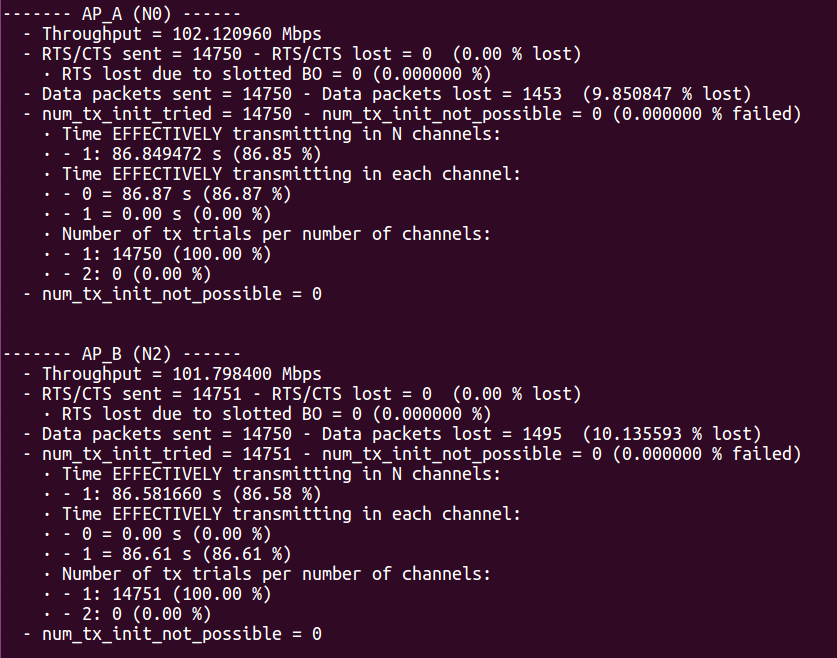
\epsfig{file=images/nodes_statistics_example, width=12cm}
			\caption{Example of nodes statistics in Komondor}
			\label{fig:nodes_statistics_example}
		\end{figure}
		
		\begin{figure}[h!]
			\centering
			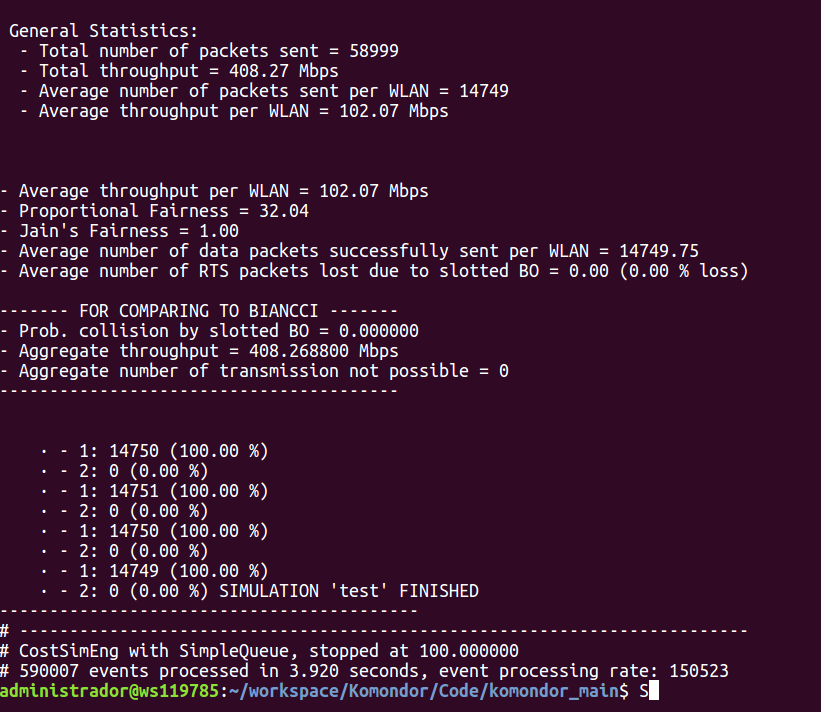
\epsfig{file=images/general_statistics_example, width=12cm}
			\caption{Example of system statistics in Komondor}
			\label{fig:general_statistics_example}
		\end{figure}
	
		% Logs system
		\subsubsection{Events Categorization}
		\label{section:events_categorization}	
		In order to make output results more understandable, logs are categorized according to the event that generates it. With that, further filtering processes can be carried out by developers. Table \ref{table:event_coding} describes the codes used for each type of event.		
		% Events coding table
		\begin{table}[h!]
		\centering
		\scriptsize
		\begin{tabular}{|c|c|c|c|}
		\hline
		\textbf{Method}                            & \textbf{Type}       & \textbf{Sub-type} & \textbf{Event description}                              \\ \hline
		Setup()                                    & A                   & -                 & -                                                       \\ \hline
		\multirow{3}{*}{Start()}                   & \multirow{3}{*}{B}  & B00               & Start()                                                 \\ \cline{3-4} 
		                                           &                     & B01               & Start() end                                             \\ \cline{3-4} 
		                                           &                     & B02               & Node's info (one line)                                  \\ \hline
		\multirow{6}{*}{Stop()}                    & \multirow{6}{*}{C}  & C00               & Stop()                                                  \\ \cline{3-4} 
		                                           &                     & C01               & Stop() end                                              \\ \cline{3-4} 
		                                           &                     & C02               & Time transmitting in number of channels                 \\ \cline{3-4} 
		                                           &                     & C03               & Time transmitting in each channel                       \\ \cline{3-4} 
		                                           &                     & C04               & Packets sent                                            \\ \cline{3-4} 
		                                           &                     & C05               & Throughput                                              \\ \hline
		\multirow{14}{*}{inportSomeNodeStartTX()}  & \multirow{14}{*}{D} & D00               & inportSomeNodeStartTX()                                 \\ \cline{3-4} 
		                                           &                     & D01               & inportSomeNodeStartTX() end                             \\ \cline{3-4} 
		                                           &                     & D02               & Node N has started a TX in channels: c\_left - c\_right \\ \cline{3-4} 
		                                           &                     & D03               & Pre update channel state                                \\ \cline{3-4} 
		                                           &                     & D04               & Distance to transmitting node                           \\ \cline{3-4} 
		                                           &                     & D05               & Power received from transmitting node                   \\ \cline{3-4} 
		                                           &                     & D06               & Post update channel state                               \\ \cline{3-4} 
		                                           &                     & D07               & I am (or not) the TX destination                        \\ \cline{3-4} 
		                                           &                     & D08               & Current SINR                                            \\ \cline{3-4} 
		                                           &                     & D09               & Capacitiy                                               \\ \cline{3-4} 
		                                           &                     & D10               & Primary channel affected (or not)                       \\ \cline{3-4} 
		                                           &                     & D11               & Power sensed in primary channel                         \\ \cline{3-4} 
		                                           &                     & D12               & CCA exceeded (or not)                                   \\ \cline{3-4} 
		                                           &                     & D13               & Backoof active (or not)                                 \\ \hline
		\multirow{10}{*}{inportSomeNodeFinishTX()} & \multirow{10}{*}{E} & E00               & inportSomeNodeFinishTX()                                \\ \cline{3-4} 
		                                           &                     & E01               & inportSomeNodeFinishTX() end                            \\ \cline{3-4} 
		                                           &                     & E02               & N\%d has finished a TX in channel range: \%d - \%d      \\ \cline{3-4} 
		                                           &                     & E03               & Initial power of transmitter                            \\ \cline{3-4} 
		                                           &                     & E04               & Pre update channel state                                \\ \cline{3-4} 
		                                           &                     & E05               & Post update channel state                               \\ \cline{3-4} 
		                                           &                     & E06               & Primary channel affected (or not)                       \\ \cline{3-4} 
		                                           &                     & E07               & Power sensed in primary channel                         \\ \cline{3-4} 
		                                           &                     & E08               & CCA exceeded (or not)                                   \\ \cline{3-4} 
		                                           &                     & E09               & I am transmitting (or not)                              \\ \hline
		\multirow{6}{*}{endBackoff()}              & \multirow{6}{*}{F}  & F00               & endBackoff()                                            \\ \cline{3-4} 
		                                           &                     & F01               & endBackoff() end                                        \\ \cline{3-4} 
		                                           &                     & F02               & Channels for transmitting                               \\ \cline{3-4} 
		                                           &                     & F03               & Transmission is possible (or not)                       \\ \cline{3-4} 
		                                           &                     & F04               & Selected transmission range                             \\ \cline{3-4} 
		                                           &                     & F05               & New backoff generated                                   \\ \hline
		\multirow{3}{*}{myTXFinished()}            & \multirow{3}{*}{G}  & G00               & myTXFinished()                                          \\ \cline{3-4} 
		                                           &                     & G01               & myTXFinished() end                                      \\ \cline{3-4} 
		                                           &                     & G02               & New backoff generated                                   \\ \hline
		\end{tabular}
		\caption{Node's event logs encoding}
		\label{table:event_coding}
		\end{table}

	%%% Code Development
	\subsection{Code development}
	\label{section:code_development}		
	Here we provide some clarifications regarding code implementation, wit the aim to facilitate the Komondor's usage and manipulation to developers that may be interested.
	
		% Considerations
		\subsubsection{Main considerations}
		\label{section:development_considerations}
		% TODO: Extend this part.
		Some technical information regarding code development is worth to be mentioned to properly understand how to use and modify the Komondor simulator. So far, the main considerations to be taken into account are:		
		\begin{itemize}
		\item \textbf{Power and CCA}: power variables are stored in pW (pico watts) in order to be able to operate power magnitudes without loosing resolution\footnote{For instance., the sum of two signals of power values -85 dBm (3.162 pW) and -90 dBm (1 pW), respectively, is -83.803 dBm (4.162 pW).}. However, values are presented to the user in dBm.		
		W (-30)  - mW (0)  - uW (+30) - nW (+60) - pW (+90)\\
		$P_{\text{pw}} = 10^{\frac{P_{\text{dBm}} + 90}{10}}$
		\end{itemize}
	
		% Miscellany
		\subsubsection{Miscellaneous}
		\label{section:development_miscellany}
		% TODO: Extend this part.
			\begin{itemize}
			\item \textbf{Transmitting capability}: we have added a flag to each node that determines if it is able to transmit (1) or not (0), so that we can decide if the node is only listening or both transmitting and listening.
			\item \textbf{Progress bar}: the Komondor simulation progress bar is displayed through a \textit{printf()} command called by any node with \textit{node\_id} set to 0. If no node has \textit{node\_id} set to 0, the progress bar is not displayed.
			\end{itemize}
	
%%%%%%%%%%%%%%%
% 6. CONCLUSIONS
%%%%%%%%%%%%%%%
\section{Conclusions}
\label{section:conclusions}
In this document we provided an overview of the first version of the Komondor simulator, which aims to reproduce the basic operation of IEEE 802.11ax WLANs in addition to allow the utilization of intelligent systems. We introduced the system model considered when building the simulator, as well as the main MAC features implemented. Additionally, due to the open source nature of this project, we provided basic information of interest for developers that are expected to use or even modify this HD WLANs simulator.

Regarding the validation of the simulator, we provided a set of meaningful test scenarios to prove the proper behavior of the simulator. As shown, tests were satisfactory as the throughput computed with Komondor and the CTMN model are pretty similar, and the differences were properly justified.

This project is expected to move forward for including of novel mechanisms such as OFDMA, MU-MIMO, TPC or  CST adjustment. In addition, intelligent agents are expected to be included for making operations such as Dynamic CB (DCB).

%%% BIBLIOGRAPHY
\bibliographystyle{unsrt}
\bibliography{bib}

\end{document}